

\pagenumbering{arabic}
\renewcommand\thefigure{OA-\arabic{figure}}
\renewcommand\thetable{OA-\arabic{table}}
\renewcommand*{\thepage}{OA - \arabic{page}}
\renewcommand\thesection{Appendix \Alph{section}.}
\renewcommand\thesubsection{\Alph{section}.\arabic{subsection}}




\begin{frontmatter}

\title{The controlled choice design and private paternalism in pawnshop borrowing - ONLINE APPENDIX}
\runtitle{The controlled choice design and private paternalism}

\begin{aug}
% use \particle for den|der|de|van|von (only lc!)
% [id=?,addressref=?,corref]{\fnms{}~\snm{}\ead[label=e?]{}\thanksref{}}
%
%% e-mail is mandatory for each author
%
%%% initials in fnms (if any) with spaces
%
\author[id=au1,addressref={add1}]{\fnms{Craig}~\snm{McIntosh}\ead[label=ee1]{ctmcintosh@ucsd.edu}}
\author[id=au2,addressref={add2}]{\fnms{Isaac}~\snm{Meza}\ead[label=ee2]{isaacmezalopez@g.harvard.edu}}
\author[id=au3,addressref={add3}]{\fnms{Joyce}~\snm{Sadka}\ead[label=ee3]{jsadka@itam.mx}}
\author[id=au4,addressref={add4}]{\fnms{Enrique}~\snm{Seira}\ead[label=ee4]{enrique.seira@gmail.com}}
\author[id=au5,addressref={add5}]{\fnms{Francis J.}~\snm{DiTraglia}\ead[label=ee5]{francis.ditraglia@economics.ox.ac.uk}}

% Addresses
\address[id=add1]{%
\orgdiv{Department of Economics}
\orgname{University of California San Diego}}

\address[id=add2]{%
\orgdiv{Department of Economics}
\orgname{Harvard University}}

\address[id=add3]{%
\orgdiv{Department of Economics}
\orgname{Instituto Tecnologico Autonomo de Mexico}}

\address[id=add4]{%
\orgdiv{Department of Economics}
\orgname{Michigan State University}}

\address[id=add5]{%
\orgdiv{Department of Economics}
\orgname{University of Oxford}}
\end{aug}


\end{frontmatter}

\begin{appendix}
    

\section{Treatment Explanation Materials and Pictures}

\subsection{Materials}

\begin{figure}[!htb]
     \caption{Contract Terms Summary}
    \label{PaperSlip}
    \begin{center}
        \includegraphics[width=0.7\textwidth]{Figuras/TicketLenderP.png}
    \end{center}
    \legend{We show a sample receipt that was given to clients that got assigned to the fee-forcing contract (the font and format were changed to protect Lender's P identity). We want to highlight the salience of some items. First the title clearly indicated which contract the client has (arrow 1). Second, in the case of the fee contract it clearly indicates that there is a fee for paying late equivalent to 2\% of the value of the monthly payment (arrow 2). Third, there is a calendar for payments clearly specifying the dates and amounts to pay each month.}
\end{figure}

\begin{figure}[!htb]
     \caption{Explanatory Material}
    \label{ExplanatoryMaterial}
    \begin{center}
    \begin{subfigure}{\textwidth}
        \centering
        \includegraphics[width=0.7\textwidth]{Figuras/micas.pdf}
    \end{subfigure}
    \end{center}
    \legend{ This is a (translated) sample information slide shown to clients. The real ones were twice the size of this figure and were laminated. Different ones were shown for each treatment arm.}
\end{figure}



\subsection{Pictures}

\begin{figure}[!htb]
     \caption{Some Pawnshops}
    \label{PawnshopPicture}
    \begin{center}
    \begin{subfigure}{0.405\textwidth}
    \caption{Appraiser/tellers inside a pawnshop}
        \centering
        \includegraphics[width=\textwidth]{Figuras/empenio9_.png}
    \end{subfigure}
        \begin{subfigure}{0.45\textwidth}
    \caption{Pawnshop}
        \centering
        \includegraphics[width=\textwidth]{Figuras/empenio11_.png}
    \end{subfigure}
    
        \vspace{3ex}

    \begin{subfigure}{0.45\textwidth}
    \caption{Pawnshop}
        \centering
        \includegraphics[width=\textwidth]{Figuras/empenio2_.png}
    \end{subfigure}
    \begin{subfigure}{0.415\textwidth}
    \caption{Lost pawns which are for sale}
        \centering
        \includegraphics[width=\textwidth]{Figuras/empenio3_.png}
    \end{subfigure}
    \end{center}
   \legend{ This figure  shows pictures of pawnshops in Mexico city. They do not necessarily coincide with Lender P for confidentiality. }
\end{figure}




\begin{figure}[!htb]
     \caption{Gold buyers next to pawnshops}
    \label{GoldBuyers}
    \begin{center}
    \begin{subfigure}{.49\textwidth}
    \caption{Gold buyer next to pawnshop 1}
        \centering
        \includegraphics[width=\textwidth]{Figuras/empenio7_.png}
    \end{subfigure}
    \begin{subfigure}{.49\textwidth}
    \caption{Gold buyer next to pawnshop 1}
        \centering
        \includegraphics[width=\textwidth]{Figuras/empenio8_.png}
    \end{subfigure}
       \vspace{3ex}
       
    \end{center}
    \legend{  This figure shows pictures of gold buyers next to pawnshops in Mexico city. They do not necessarily coincide with Lender P for confidentiality. }
\end{figure}


\subsection{Descriptives consistent with overconfidence}

\vspace{.2in}
\begin{figure}[!htb]
    \caption{Behavior of borrowers who lost their pawn}
    \label{proxy_naive}
    \begin{center}
    \begin{subfigure}{0.40\textwidth}
        \caption{Elapsed days to first payment}
        \centering
        \includegraphics[width=\textwidth]{Figuras/hist_firstdays_default.pdf}
    \end{subfigure}
    \begin{subfigure}{0.40\textwidth}
        \caption{Elapsed days to last payment}
        \centering
        \includegraphics[width=\textwidth]{Figuras/hist_days_default.pdf}
    \end{subfigure}
        \begin{subfigure}{0.40\textwidth}
        \caption{Payments as \% of loan}
        \centering
        \includegraphics[width=\textwidth]{Figuras/hist_percpay_default.pdf}
    \end{subfigure}
    \begin{subfigure}{0.40\textwidth}
        \caption{Number of payments}
        \centering
        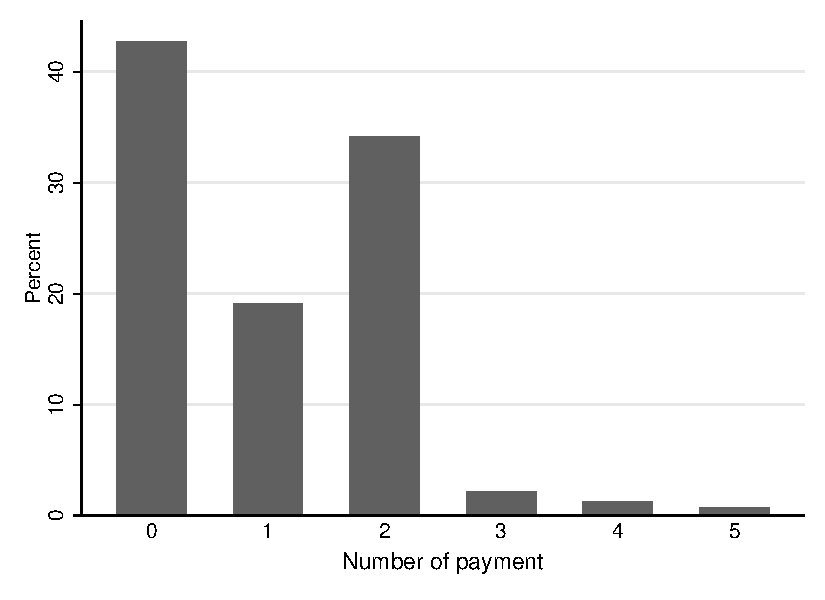
\includegraphics[width=\textwidth]{Figuras/hist_numpay_default.pdf}
    \end{subfigure}
    \end{center}
       \legend{ This figure provides more details on the behavior of clients who were assigned to the control group and did not recover their pawn. Panel (a) shows a histogram of days elapsed from the pawn to the first payment, while panel (b) displays a histogram of days elapsed until the last payment. Some borrowers make payments after day 105, the end of the grace period: if they pay all interest owed, they can ``restart'' the loan. This amounts to starting a new loan with the same conditions and same pawn. Panel (c) shows a histogram of the fraction of the loan paid, while panel (d) presents a barplot of the number of times that borrowers went to the branch to make payments.}
      %\textit{Do file: }  \texttt{hist\_den\_default.do}
\end{figure}

    
\section{Internal Validity}

\subsection{Survey}   \label{app:survey_data}

We now present analysis of the extent to which the survey-responding sample is representative and balanced.
Table \ref{SS_cond_survet} presents information about survey non-response.
Panel A is a balance table that compares loan amount and day of the week across treatment arms for the subset of borrowers who responded to at least one survey question.
The p-values in the fourth column are for the F-test of no difference of means across treatment arms. 
Panel B presents response-rates by question for each arm of the experiment, along with p-values for the F-test of no difference in question-specific response rates across treatment arms. 
This panel uses data from participants who answered at least one survey question and went on to pawn on the same day as their survey response.
From the table, we see that loan amount and weekday are balanced across treatment arms among survey respondents and that response rates are likewise stable across treatment arms.
Table \ref{TUT_cond_survet} shows how the estimated TUT effect changes if we restrict our estimation sample based on survey response.
The first row of the table presents TUT results for the financial cost outcome, while the second presents corresponding results for the APR outcome.
In each row, column (1) presents the full-sample TUT estimate and standard error while the remaining columns restrict the sample to borrowers who answered a particular survey question or set of questions.
For example, column (4) presents results for borrowers who answered the two questions needed to compute our measure of ``present bias'' discussed in the next paragraph, while column (9) present results restricted to participants who disclosed their sex. 
As seen from the table, our TUT estimates are quite stable across sub-samples defined by survey response.
In each case they are positive and of the same magnitude as the corresponding full-sample estimate, although statistical significance varies depending on the size of the corresponding sub-sample. 
For these reasons, we are comfortable relying on data for survey respondents in the empirical exercises that follow.
In exercises that rely on a single survey question, we use data for every borrower who answered that question.
In the random forest exercises described below, we use data for every borrower who answered at least one survey question.



\begin{table}[!htb]
\caption{Baseline survey questions (translated to English)}
\label{baseline_survey}
\begin{center}
\scriptsize{% Table generated by Excel2LaTeX from sheet 'transcribed'
\begin{tabular}{cl}
\toprule
      & \textbf{Baseline Survey} \\
\midrule
\midrule
1     & \textbf{Your pawn was:} \\
      & (a) Inherite, (b) a gift, (c) bought by me, (d) lend to me, (e) other \_\_\_\_\_\_\_\_\_\_\_\_ \\
2     & \textbf{Mark with an "X" in the line below how likely is that you recover your pawn. } \\
      & \textbf{Where 0 is impossible and 100 is completely certain} \\
3     & \textbf{How much would you sell the item you want to pawn for?       \_\_\_\_\_\_\_\_\_\_\_\_\_\_ pesos} \\
4     & \textbf{Gender      } \\
5     & \textbf{Age} \\
6     & \textbf{Civil Status } \\
      & (a) married, (b) single, (c) divorced, (d) widowed \\
7     & \textbf{Work status} \\
      & (a) employed, (b) own business, (c) houseshores, (d) don't work, (e) retired, (f) study \\
8     & \textbf{Education} \\
      & (a) no formal education, (b) primary, (c) middle school, (d) highschool, (e) more than highschool \\
9     & \textbf{In the last month, did a friend or family member asked you for money?} \\
      & (a) yes  (b) no \\
10    & \textbf{What would you like to have: 100 pesos tomorrow or 150 pesos in one month?} \\
11    & \textbf{How often do you feel stressed by your economic situation?} \\
      & (a) always, (b) very often, (c) sometimes, (d) never \\
12    & \textbf{What is the main reason you want to pawn?} \\
      & (a) Need the money because somebody in my family lost his/her job \\
      & (b) Need the money to pay for a sickness in the family \\
      & (c) Need the money for an urgent expense \\
      & (d) Need the money for some non urgent expense. \\
13    & \textbf{How stressed do you feel from the situation that led to to pawn?} \\
      & (a) very stressed, (b) somwhat stressed, (c) a little stressed, (d) not stressed  \\
14    & \textbf{In 3 months, I expect to have a  \_\_\_\_\_\_\_\_\_\_\_\_\_\_\_\_ situation} \\
      & (a) better, (b) similar,  (c) worse \\
15    & \textbf{Have you panwned before?} \\
      & (a) yes  (b) no \\
16    & \textbf{How many times have you pawned on a Lender P branch?} \\
      & (a) NO\_\_\_    (b)  1-2 times \_\_\_    (c) 3-5 times\_\_\_\_   (d) More than 5\_\_\_\_ \\
17    & \textbf{If you are saving money and a family member wants to use it for something } \\
      & (a) I would only give him the money for an urgent expenze \\
      & (b) I would give him the money even if it was not an urgent expense \\
      & (c) I would not give him/her the money regardless \\
      & (d) No one would ask me for my money \\
18    & \textbf{Do you make an expenses budget for the month ahead of time?} \\
      & (a) always, (b) very often, (c) sometimes, (d) never \\
19    & \textbf{Do you have other items you could pawn?} \\
      & (a) yes  (b) no \\
20    & \textbf{Do you have savings?} \\
      & (a) yes  (b) no \\
21    & \textbf{Do you participate in a ROSCA?} \\
      & (a) yes  (b) no \\
22    & \textbf{Is it common that family or friends ask for money?} \\
      & (a) yes  (b) no \\
23    & \textbf{How much did you spend to come to the branch today?    \$\_\_\_\_\_\_\_\_\_\_\_\_\_\_ pesos} \\
24    & \textbf{How much time does it usually take to come to this branch?    \_\_\_\_\_\_\_\_\_\_\_} \\
25    & \textbf{How much does your family spend in a normal week?   \$\_\_\_\_\_\_\_\_\_\_\_\_\_\_ pesos} \\
26    & \textbf{How much do you manage to save in a normal week?   \$\_\_\_\_\_\_\_\_\_\_\_\_\_\_ pesos} \\
27    & \textbf{Does it happen to you that you spend more than you wanted because you fall into temptation?} \\
      & (a) never, (b) almost never, (c) sometimes, (d) very often \\
28    & \textbf{In the last 6 months, has it happened that at some point you lacked money to pay} \\
      & (a) rent?    (b) food    (c)food   (d) medicine  (e) electricity   (f) heating   (g) telephone    (i) water \\
29    & \textbf{What would you like to have: 100 pesos in 3 months or 150 pesos in four months?} \\
30    & \textbf{Would you like to receive (free) reminders for upcomming payments?} \\
      & (a) yes  (b) no \\
\bottomrule
\end{tabular}%
}
\end{center}
\legend{ Translation of the baseline questionnaire.}
\end{table}


\begin{figure}[!htb]
     \caption{Box-plot across arms}
    \label{boxplot_attrition}
    \begin{center}
    \begin{subfigure}{0.45\textwidth}
    \caption{Number of pawns}
        \centering
        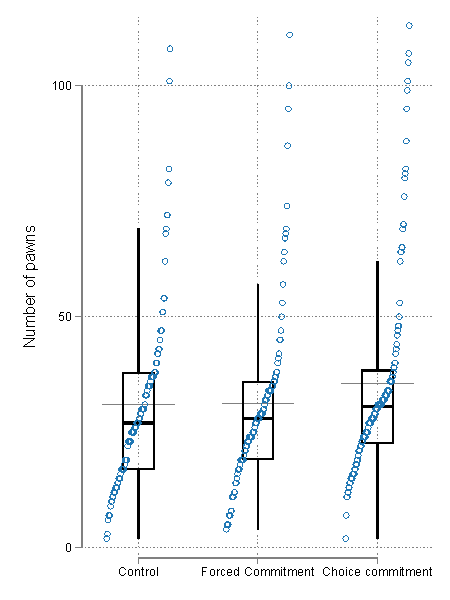
\includegraphics[width=\textwidth]{Figuras/box_plot_num_pawns.pdf}
    \end{subfigure}
        \begin{subfigure}{0.45\textwidth}
    \caption{Number of borrowers}
        \centering
        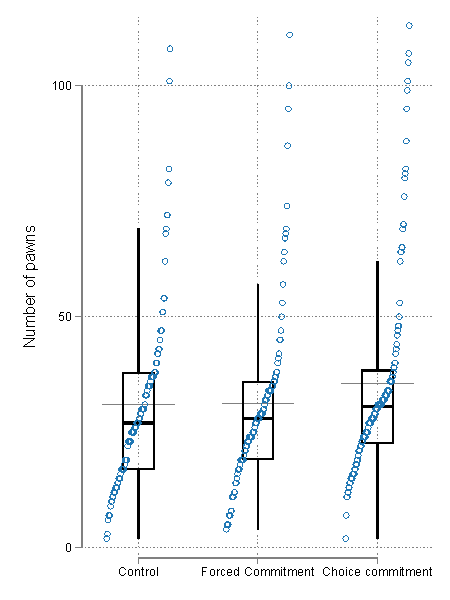
\includegraphics[width=\textwidth]{Figuras/box_plot_num_pawns.pdf}
    \end{subfigure}
    \end{center}
    \legend{ This figure presents box-plot for the number of pawns and borrowers per branch-day across different arms. The solid black line represent the median, while the gray line represent the mean. The dots on top of the box-plot represent an implicit CDF. }
\end{figure}




\begin{table}[!htb]
\caption{Balance conditional on survey response and question-by-question response rates by treatment arm}
\label{SS_cond_survet}
\begin{center}
\scriptsize{% Table generated by Excel2LaTeX from sheet 'SS_cond_survey'
\begin{tabular}{lcccc}
\toprule
      &       & \multicolumn{3}{c}{Commitment arms} \\
\cmidrule{3-5}      & \multicolumn{1}{p{4.5em}}{Control} & \multicolumn{1}{p{4.93em}}{Forced} & \multicolumn{1}{p{3.43em}}{Choice} & \multicolumn{1}{p{3.43em}}{p-value} \\
\midrule
      & \multicolumn{4}{c}{Panel A : Administrative Data (conditional on survey)} \\
\midrule
\midrule
Loan amount  & 2199  & 2196  & 2216  & 0.98 \\
      & (86)  & (106) & (81)  &  \\
Weekday & 0.88  & 0.89  & 0.85  & 0.8 \\
      & (0.045) & (0.038) & (0.045) &  \\
\midrule
Obs   & 1386  & 1469  & 1982  &  \\
\midrule
      & \multicolumn{4}{c}{Panel B : Survey Data - response rate} \\
\midrule
\midrule
Subjective value & 0.73  & 0.69  & 0.71  & 0.39 \\
      & (0.022) & (0.024) & (0.024) &  \\
Trouble paying bills & 0.49  & 0.48  & 0.44  & 0.29 \\
      & (0.023) & (0.022) & (0.022) &  \\
Present bias & 0.43  & 0.44  & 0.39  & 0.17 \\
      & (0.02) & (0.02) & (0.02) &  \\
Makes budget & 0.55  & 0.56  & 0.53  & 0.56 \\
      & (0.023) & (0.023) & (0.019) &  \\
Subj. pr. of recovery & 0.74  & 0.72  & 0.74  & 0.71 \\
      & (0.024) & (0.025) & (0.025) &  \\
Pawn before & 0.55  & 0.57  & 0.53  & 0.57 \\
      & (0.023) & (0.024) & (0.02) &  \\
Age   & 0.54  & 0.55  & 0.52  & 0.59 \\
      & (0.023) & (0.023) & (0.018) &  \\
Woman & 0.58  & 0.59  & 0.58  & 0.93 \\
      & (0.025) & (0.024) & (0.02) &  \\
+ High-school & 0.54  & 0.55  & 0.51  & 0.39 \\
      & (0.025) & (0.025) & (0.019) &  \\
\midrule
Obs   & 1386  & 1469  & 1982  &  \\
\bottomrule
\bottomrule
\end{tabular}%
}
\end{center}
\legend{ Panel A of this table presents the same information as Panel A of Table \ref{SS}, but restricts attention to the subsample of borrowers who answered at least one question in our baseline survey. Conditional on survey response, loan amount and weekday are balanced across treatment arms. Panel B presents response rates to each individual survey question across treatment arms, along with p-values for the F-test of no difference in response rates across survey arms. This panel uses data for borrowers who pawned on the same day as their survey response. }


%\textit{Do file: } \texttt{ss\_att.do}
\end{table}



\begin{landscape}
\begin{table}[!htb]
\caption{Survey Non-response: TUT estimates for respondents to each survey question.}
\label{TUT_cond_survet}
\begin{center}
\scriptsize{% Table generated by Excel2LaTeX from sheet 'tut_cond_survey'
\begin{tabular}{lcccccccccc}
\toprule
      & Full-sample & Subjective value & Trouble paying bills & Present bias & Makes budget & Subj. pr. of recovery & Pawn before & Age   & Woman & + High-school \\
\midrule
      & (1)   & (2)   & (3)   & (4)   & (5)   & (6)   & (7)   & (8)   & (9)   & (10) \\
\midrule
\midrule
Apr \% benefit & 10.3*** & 10.4*** & 11.3*** & 12.0*** & 10.4*** & 11.2*** & 10.5*** & 11.0*** & 11.5*** & 11.0*** \\
      & (2.44) & (2.36) & (2.59) & (2.64) & (2.68) & (2.29) & (2.67) & (2.89) & (2.91) & (2.84) \\
      &       &       &       &       &       &       &       &       &       &  \\
\midrule
      & (11)  & (12)  & (13)  & (14)  & (15)  & (16)  & (17)  & (18)  & (19)  & (20) \\
\midrule
\midrule
FC benefit TuT & 187.1*** & 185.6*** & 143.7** & 183.9** & 154.9** & 181.2*** & 141.4** & 160.7** & 138.0** & 129.0* \\
      & (50.7) & (58.0) & (67.6) & (81.9) & (69.8) & (60.7) & (68.5) & (74.5) & (69.1) & (72.5) \\
      &       &       &       &       &       &       &       &       &       &  \\
\midrule
Observations & 6304  & 4465  & 2948  & 2613  & 3433  & 4625  & 3468  & 3393  & 3677  & 3352 \\
\bottomrule
\bottomrule
\end{tabular}%
}
\end{center}
\legend{ Some borrowers did not respond to our survey; others only completed part of the survey.
This table computes the TUT effect for a number of sub-groups by survey response, and compares them against the overall TUT effect.
The top panel uses financial cost as the outcome variable, while the bottom panel uses APR.
Each group is defined by the borrowers who responded to a particular \emph{subset} of the survey questions. 
For example, column (4) computes TUT effects for the subgroup of borrowers who responded to the two questions needed to compute our measure of present bias, while column (8) computes the TUT for the subgroup of borrowers who provided their age.
The bottom row of the table counts the number of borrowers in each category.
TUT estimates are quite stable across sub-groups and generally similar to the full-sample estimates.
Because standard errors increase as sample size falls, some of the sub-group estimates are not statistically significant.}
%\textit{Do file: } \texttt{tut_cond_survey.do}
\end{table}
\end{landscape}



\section{Main treatment effects: Additional material}


\begin{landscape}
\subsection{Multiple loans}

\begin{table}[!htb]
\caption{Multiple-loans robustness check}
\label{multiple_loans}
\begin{center}
\scriptsize{% Table generated by Excel2LaTeX from sheet 'multiple_loans'
\begin{tabular}{lcccccccccccccc}
\toprule
      & \multicolumn{4}{c}{First visit (Baseline approach)} &       & \multicolumn{4}{c}{Multiple visits - multiple treatments} &       & \multicolumn{4}{c}{First treatment (ITT)} \\
\cmidrule{7-10}\cmidrule{12-15}      & FC    & APR   & Recovery & Default &       & FC    & APR   & Recovery & Default &       & FC    & APR   & Recovery & Default \\
\midrule
      & (1)   & (2)   & (3)   & (4)   &       & (5)   & (6)   & (7)   & (8)   &       & (9)   & (10)  & (11)  & (12) \\
\midrule
\midrule
Forced Commitment & -202.8*** & -0.11*** & 0.14*** & -0.065*** &       & -175.2*** & -0.078*** & 0.099*** & -0.032 &       & -159.1*** & -0.086*** & 0.11*** & -0.051*** \\
      & (48.1) & (0.019) & (0.025) & (0.023) &       & (42.8) & (0.017) & (0.021) & (0.020) &       & (38.6) & (0.015) & (0.021) & (0.019) \\
Choice Commitment & -39.6 & -0.0089 & 0.0094 & -0.024 &       & -34.4 & 0.0028 & 0.00054 & -0.0049 &       & -31.5 & -0.017 & 0.029 & -0.032* \\
      & (49.8) & (0.019) & (0.022) & (0.021) &       & (43.5) & (0.016) & (0.018) & (0.018) &       & (40.4) & (0.014) & (0.018) & (0.018) \\
      &       &       &       &       &       &       &       &       &       &       &       &       &       &  \\
\midrule
Observations & 6304  & 6304  & 6304  & 6304  &       & 8519  & 8519  & 8519  & 8519  &       & 8813  & 8813  & 8813  & 8813 \\
R-sq  & 0.013 & 0.031 & 0.019 & 0.013 &       & 0.016 & 0.032 & 0.018 & 0.010 &       & 0.016 & 0.031 & 0.020 & 0.015 \\
Control Mean & 941.3 & 0.57  & 0.43  & 0.44  &       & 905.7 & 0.54  & 0.46  & 0.42  &       & 904.7 & 0.55  & 0.44  & 0.44 \\
\bottomrule
\bottomrule
\end{tabular}%
}
\end{center}
 \legend{ An additional empirical issue generated by repeat pawning is the question of how to handle the treatment status of those who take multiple loans within the experiment.  43\% of borrowers take more than one loan within the study period, and 19\% are assigned multiple treatment statuses on their different loans.  The issue of sequential endogenous treatments has been extensively studied in the context of school lotteries, where the convention is to use the treatment status from the first exposure (ITT) \citep{cullen2006effect, abdulkadirouglu2011accountability}.\\
 This table provides robustness for our main results for different ways to handling the multiplicity of loans. Columns 1-4 repeat the main analysis of financial cost and APR using the baseline approach from our main results,i.e. it only considers the first visit, while allowing multiple loans for the same-day. Columns 5-8 considers all loans including dummies for the order of pawns for an individual, essentially making the identification within-order.  Columns 9-12 pursue the ITT strategy of always assigning the first treatment status to all subsequent pawns. The core treatment effects are robust to any of these ways of handling repeat pawning.  }
 
%\textit{Do file: } \texttt{multiple\_loans.do}
\end{table}


\end{landscape}


\begin{figure}[!htb]
    \caption{Determinants of choice}
    \label{determinants_choose}
    \begin{center}
    \begin{subfigure}{0.5\textwidth}
        \centering
        \includegraphics[width=\textwidth]{Figuras/determinants_choose_commitment.pdf}
    \end{subfigure}
    \end{center}
      \legend{  The above figure shows the determinants in a bivariate and multivariate OLS regression of choosing commitment. Choice commitment is a binary variable equal to one, whenever subjects choose the forced commitment contract in the choice arm. }
%\textit{Do file: } \texttt{determinants_choice.do}       
\end{figure}


\vspace{.2in}
\begin{figure}[!htb]
    \caption{Histogram of payments}
    \label{hist_payments}
    \begin{center}
    \begin{subfigure}{0.32\textwidth}
        \caption{Status-quo}
        \centering
        \includegraphics[width=\textwidth]{Figuras/hist_payments_sq.pdf}
    \end{subfigure}
    \begin{subfigure}{0.32\textwidth}
        \caption{Forced commitment}
        \centering
        \includegraphics[width=\textwidth]{Figuras/hist_payments_fc.pdf}
    \end{subfigure}
    \begin{subfigure}{0.32\textwidth}
        \caption{Choice commitment}
        \centering
        \includegraphics[width=\textwidth]{Figuras/hist_payments_cc.pdf}
    \end{subfigure}    
    \end{center}
     \legend{ This figure shows the schedule of payments for each treatment arm. In other words it records the time after the loan origination when the borrower makes a payment toward recovery of the pawn. We can see that for both the Forced commitment and Choice commitment arm, payments are bunching at the 30 and 60 days, while most payments are done around the due date of the loan (90 days).}
     
      %\footnotesize{ \textit{Do file: }  \texttt{hist\_payments.do}}
\end{figure}




\subsection{Censoring} \label{App_censoring}


Some loans in our sample are ``censored'' in that they continue beyond our observation period.
For these loans, we do not know whether the borrower ultimately defaulted or recovered her pawn.
In this appendix, we show that our main results are robust to different ways of addressing censoring.

Our main results, presented above, make no assumption on the default/recovery status of this loans. However, we compute the Financial Cost \& APR considering all the payments done so far. We now consider some alternative approaches. \\
  

One way of considering the effect that this issue could have on our results is to make extreme assumptions about the outcome of these loans in the treatment and control so as to bound the possible influence of censoring.  In Table \ref{bounding_censoring} we compare the Forced and Control arms, making the bracketing assumptions about repayment on censored loans.  Panel A assumes all censored loans are repaid, and Panel D that all default. Because forced commitment causes borrowers to make payments earlier than they otherwise would have, In Panel A we make a conservative assumption. To see why, suppose for the sake of argument that commitment affects payment timing, but does not not default.
In other words, suppose that treatment makes censoring \emph{less likely} but has no effect on uncensored outcomes. 
If we were to treat all outstanding loans as defaults--the opposite of our convention--this would artificially inflate the rate of default among control loans relative to treatment loans.

Panel B provides the lower bound for the treatment effect by assuming censored control loans are always repaid and treatment loans never are, and Panel C the upper bound by making the reverse assumption.  Comfortingly, even with these extreme assumptions the significance on the main treatment effects never flips and treatment effects on financial cost and interests payments remain negative and significant in all scenarios.  So there appears to be no scope for the censoring issue to overturn our main results. 



Finally, Panel E of this table conducts a lasso logit prediction model that uses all of the available information on loans that were completed to predict the outcome of loans that were not.  This is a best guess of the outcome on censored loans.  Using this prediction, we replicate the main experimental results and find that the treatment effect on financial cost increases from -204 (main results) to -264 (censored loans predicted), and the APR from -11\% to -17\%.  Hence, while the censoring issue does have a substantial influence on the magnitude of our estimated treatment effects, these  checks confirm that a) the core results are robust to censoring, and b) the headline approach that we take to the issue is conservative and is likely understating the true magnitude of impacts.


\begin{table}[!htb]
\caption{Bounding censoring} 
\label{bounding_censoring}
\begin{center}
\resizebox{0.9\textwidth}{!}{
\scriptsize{% Table generated by Excel2LaTeX from sheet 'censoring_imp'
\begin{tabular}{lcccccc}
\toprule
      & FC    & Interest pymnt & Principal pymnt & Lost pawn value & Default & APR \\
\midrule
      & \multicolumn{6}{c}{Panel A : $\quad$ Control  = 0           $\quad\quad$                  Forced Commitment = 0} \\
\midrule
\midrule
      & (1)   & (2)   & (3)   & (4)   & (5)   & (6) \\
\midrule
\midrule
Forced commitment  & -408.3*** & -191.8*** & -0.42 & -248.1** & -0.063*** & -0.37*** \\
      & (107.2) & (37.6) & (3.01) & (101.4) & (0.023) & (0.078) \\
      &       &       &       &       &       &  \\
\midrule
Observations & 3724  & 3724  & 3724  & 3724  & 3724  & 3724 \\
R-sq  & 0.012 & 0.025 & 0.004 & 0.012 & 0.019 & 0.022 \\
Control Mean & 1898.1 & 593.5 & 5.75  & 1304.7 & 0.43  & 1.88 \\
\midrule
\midrule
      &       &       &       &       &       &  \\
\midrule
      & \multicolumn{6}{c}{Panel B : $\quad$ Control  = 0         $\quad\quad$                    Forced Commitment = 1} \\
\midrule
\midrule
      & (7)   & (8)   & (9)   & (10)  & (11)  & (12) \\
\midrule
\midrule
Forced commitment  & -226.1** & -207.7*** & 1.38  & -50.0 & 0.0094 & 0.095 \\
      & (110.8) & (37.4) & (3.45) & (103.3) & (0.024) & (0.096) \\
      &       &       &       &       &       &  \\
\midrule
Observations & 3724  & 3724  & 3724  & 3724  & 3724  & 3724 \\
R-sq  & 0.009 & 0.026 & 0.004 & 0.009 & 0.014 & 0.014 \\
Control Mean & 1898.1 & 593.5 & 5.75  & 1304.7 & 0.43  & 1.88 \\
\midrule
\midrule
      &       &       &       &       &       &  \\
\midrule
      & \multicolumn{6}{c}{Panel C : $\quad$ Control  = 1        $\quad\quad$                     Forced Commitment = 0} \\
\midrule
\midrule
      & (13)  & (14)  & (15)  & (16)  & (17)  & (18) \\
\midrule
\midrule
Forced commitment  & -804.2*** & -140.4*** & -2.33 & -695.5*** & -0.21*** & -1.17*** \\
      & (113.3) & (34.1) & (3.16) & (100.8) & (0.023) & (0.10) \\
      &       &       &       &       &       &  \\
\midrule
Observations & 3724  & 3724  & 3724  & 3724  & 3724  & 3724 \\
R-sq  & 0.022 & 0.020 & 0.004 & 0.022 & 0.053 & 0.082 \\
Control Mean & 2272.4 & 545.9 & 7.69  & 1726.5 & 0.57  & 2.62 \\
\midrule
\midrule
      &       &       &       &       &       &  \\
\midrule
      & \multicolumn{6}{c}{Panel D : $\quad$ Control  = 1       $\quad\quad$                      Forced Commitment = 1} \\
\midrule
\midrule
      & (19)  & (20)  & (21)  & (22)  & (23)  & (24) \\
\midrule
\midrule
Forced commitment  & -622.0*** & -156.3*** & -0.53 & -497.3*** & -0.13*** & -0.71*** \\
      & (117.3) & (33.8) & (3.58) & (103.1) & (0.024) & (0.12) \\
      &       &       &       &       &       &  \\
\midrule
Observations & 3724  & 3724  & 3724  & 3724  & 3724  & 3724 \\
R-sq  & 0.015 & 0.021 & 0.003 & 0.013 & 0.028 & 0.030 \\
Control Mean & 2272.4 & 545.9 & 7.69  & 1726.5 & 0.57  & 2.62 \\
\midrule
\midrule
      &       &       &       &       &       &  \\
\midrule
      & \multicolumn{6}{c}{Panel E : $\quad$ Prediction with lasso-logit model} \\
\midrule
\midrule
      & (25)  & (26)  & (27)  & (28)  & (29)  & (30) \\
\midrule
\midrule
Forced commitment  & -529.7*** & -172.4*** & -1.26 & -389.4*** & -0.12*** & -0.62*** \\
      & (120.5) & (37.4) & (3.22) & (110.2) & (0.025) & (0.11) \\
Choice commitment & -61.5 & -30.6 & -4.52 & -32.3 & -0.016 & -0.039 \\
      & (124.6) & (42.0) & (2.78) & (114.5) & (0.023) & (0.11) \\
      &       &       &       &       &       &  \\
\midrule
Observations & 6304  & 6304  & 6304  & 6304  & 6304  & 6304 \\
R-sq  & 0.012 & 0.022 & 0.003 & 0.009 & 0.016 & 0.024 \\
Control Mean & 2077.4 & 567.5 & 7.51  & 1509.9 & 0.51  & 2.28 \\
\bottomrule
\bottomrule
\end{tabular}%
}
}
\end{center}
 
 \legend{  Given the censored loans, i.e. loans that have not finished by the end of the observation period, we estimate `a la Manski' bounds for these loans, meaning that we impute all loans to either \emph{default}$=1$ or \emph{recovery}$=0$ depending on the treatment arm. Different panels perform different imputations for the censored loans for all possible combinations for the imputation, and computes the ATE for the same outcomes of Table \ref{main_impact_table}. Panel A, for instance, assumes that all outstanding loans are fully payed. Panel B is the most conservative imputation since it assumes all outstanding loans in the control arm are payed, while all the outstanding loans in the forced commitment arm default. Panel C, on the other hand, is the most optimistic scenario opposite to that of Panel B. Panel D assumes all remaining loans default. The last panel makes the imputation to the censored loans according to the best prediction using a piecewise lasso logit model for default. In concrete, we build two logit models with lasso regularization, depending whether the loan duration is less than 220 days (two cycles) or more than 220 days. For prediction we use the former whenever the last recorded payment was done within 220 days, and the latter otherwise. Both models includes loan characteristics (loan size, branch), and payment behavior (loan duration so far, days to first payment, \% of first payment, \% of payments at 30, 60, 90, and 105 days, and \% of interest payed at 105 days), but the latter model also includes \% of payments at 150, 180, and 210 days. This predictive model achieves an accuracy rate of 92\% both in-sample and out-of-sample.
 Note that in all panels we maintain significant results for Financial Cost as dependent variable, while only in the most conservative scenario (Panel B) we lose significance for the APR outcome. }
 \end{table}
 
\begin{figure}[!htb]
        \caption{Interpolation on bounding censoring}
    \label{interpolation_censoring_imp}
    \begin{center}
   \begin{subfigure}{0.49\textwidth}
   \caption{Significance area for APR}
        \centering
        \includegraphics[width=\textwidth]{Figuras/frontera_sig_apr.pdf}
    \end{subfigure}     
    \begin{subfigure}{0.49\textwidth}
   \caption{Significance area for Default }
        \centering
        \includegraphics[width=\textwidth]{Figuras/frontera_sig_def_imp.pdf}
    \end{subfigure} 
    \end{center}
     \legend{  The next figure aims to answer the following question: For how many loans in the control arm can we impute recovery, and for how many in the treatment arm can we impute default and still have significance?
     This figure shows exactly the boundary separating significance when we vary the percentage of imputed censored loans with recovery and default respectively for control and treatment. Each corner in the square will correspond to one of the panels from the Table \ref{bounding_censoring}. For instance, the origin is the best-case scenario (Panel C) and the point (100,100) (Panel B) is the worst-case scenario. Thus we can think of this graph as an `interpolation' from the four extreme cases. The `x' indicates the proportions imputed by the lasso logit model, and the different lines correspond to setting different significance levels. We do not include the plot for financial cost, since for any imputation we still have significant results.}

     %\textit{Do file: }  \texttt{interpolation_censoring_imp.do}
\end{figure}





\begin{figure}[!htb]
        \caption{Survival graph}
    \label{survival_graph}
    \begin{center}
   \begin{subfigure}{0.49\textwidth}
   \caption{Ended contract}
        \centering
        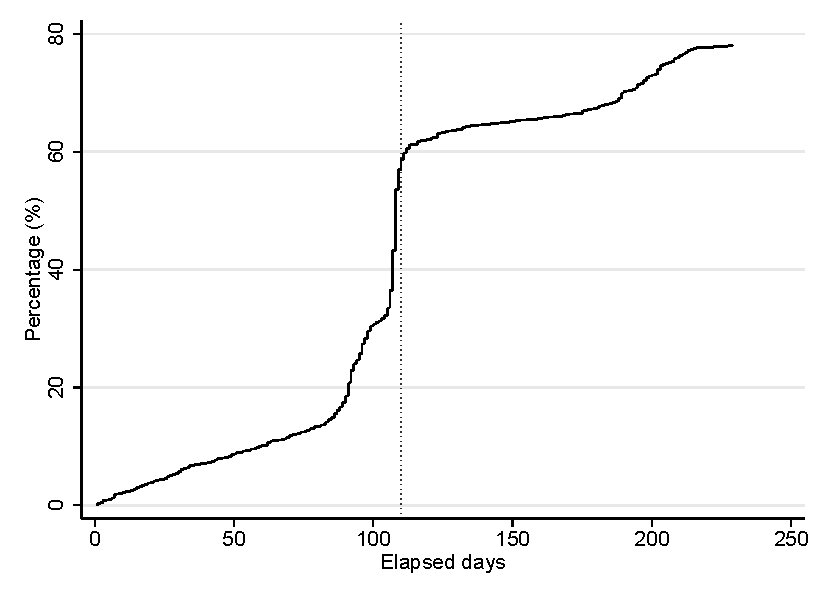
\includegraphics[width=\textwidth]{Figuras/survival_graph_ended.pdf}
    \end{subfigure} 
   \begin{subfigure}{0.49\textwidth}
   \caption{Recovery}
        \centering
        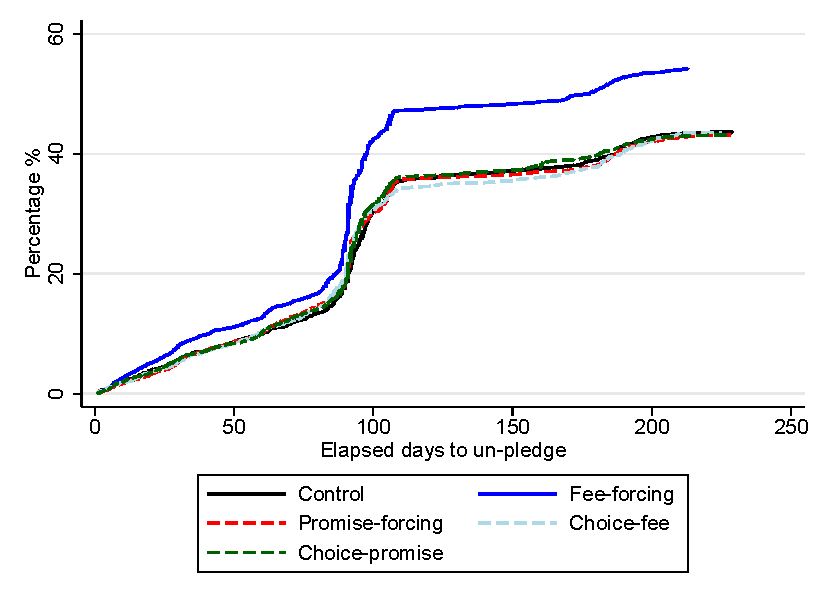
\includegraphics[width=\textwidth]{Figuras/survival_graph_unpledge.pdf}
    \end{subfigure}     
    \end{center}
     \legend{  This Figure shows the CDF of loan completion either default or recovery in Panel (a), or loan recovery in Panel (b), by the number of days since first pawn.}
     %\textit{Do file: }  \texttt{survival\_graph.do}
\end{figure}

\begin{figure}[!htb]
        \caption{\% of payment over time}
    \label{porc_payment_over_time}
    \begin{center}
   \begin{subfigure}{0.49\textwidth}
        \caption{Unconditional}
        \centering
        \includegraphics[width=\textwidth]{Figuras/cumulative_porc_pay_time.pdf}
    \end{subfigure} 
   \begin{subfigure}{0.49\textwidth}
        \caption{Conditional on default}
        \centering
        \includegraphics[width=\textwidth]{Figuras/cumulative_porc_pay_time_default.pdf}
    \end{subfigure}     
    \end{center}
     \legend{  This Figure shows the accumulated percentage of recovery in time by treatment arm. }
     %\textit{Do file: }  \texttt{cumulative\_porc\_pay\_time.do}
\end{figure}


















\section{Alternative explanations}

\subsection{Learning}

Table \ref{learning_table} presents information about borrowers' \emph{future} pawning behavior as a function of treatment assignment. Column (1) considers the 228 clients who returned only a second time to pawn again at a day/branch that was randomly assigned to the choice arm. Each of the two rows in this column presents a difference of mean commitment take-up rates, and associated standard error. The first row compares those who were \emph{initially} assigned to forced commitment against those where were assigned to control; the second row compares those who were initially assigned to the choice commitment arm to those who were assigned to the other two arms. In each case, there is no statistically discernible difference in the rates of commitment take-up. Granted, this is a selected sample because the decision to pawn again is potentially endogenous to the initial treatment allocation. For this reason, Column (2) considers the full sample of 4441 borrowers by re-defining the outcome variable to be an indicator for returning to pawn again at a branch/day when commitment was offered \emph{and} choosing commitment. This composite outcome variable is not subject to the sample selection problem (although it is directly driven by the decision to repeat borrow). The comparison in the two rows remains the same: forced commitment versus control in row one and choice commitment versus forced arms in row two. Again, there is no statistically discernible difference in commitment take-up rates in either row. While these exercises cannot completely exclude the possibility that learning plays a role, they provide no indication that the lack of voluntary compliance is simply a matter of inexperience with commitment.


\begin{table}[!htb]
        \caption{Effect of Prior Assignment on Subsequent Choice}
    \label{learning_table}
\begin{center}
\scriptsize{% Table generated by Excel2LaTeX from sheet 'learning_exp'
\begin{tabular}{lccccccccc}
\toprule
      & \multicolumn{4}{c}{Choose commitment} &       & \multicolumn{4}{c}{Ever chooses commitment} \\
\cmidrule{2-5}\cmidrule{7-10}$t-1$ & (1)   & (2)   & (3)   & (4)   &       & (5)   & (6)   & (7)   & (8) \\
\midrule
\midrule
Forced commitment & -0.0010 & -0.0076 & 0.036 & 0.030 &       & 0.0015 & 0.0043 & 0.0037 & 0.0068 \\
      & (0.044) & (0.058) & (0.036) & (0.053) &       & (0.0032) & (0.0050) & (0.0029) & (0.0047) \\
Choice : Status-quo & -0.032 & -0.026 & -0.054 & -0.054 &       & -0.0021 & -0.0013 & -0.00096 & 0.000025 \\
      & (0.040) & (0.061) & (0.066) & (0.081) &       & (0.0026) & (0.0038) & (0.0023) & (0.0037) \\
Choice : commitment & 0.51*** & 0.35* & 0.40*** & 0.25  &       & 0.031* & 0.027 & 0.026* & 0.023 \\
      & (0.16) & (0.20) & (0.13) & (0.16) &       & (0.016) & (0.019) & (0.014) & (0.018) \\
Default (D) &       & -0.035 &       & -0.024 &       &       & -0.0015 &       & 0.00024 \\
      &       & (0.046) &       & (0.044) &       &       & (0.0037) &       & (0.0034) \\
Forced commitment\#(D) &       & -0.0063 &       & -0.0071 &       &       & -0.0067 &       & -0.0069 \\
      &       & (0.074) &       & (0.077) &       &       & (0.0057) &       & (0.0056) \\
Choice : Status-quo\#(D) &       & -0.0064 &       & -0.034 &       &       & -0.0016 &       & -0.0017 \\
      &       & (0.067) &       & (0.064) &       &       & (0.0045) &       & (0.0044) \\
Choice : commitment\#(D) &       & 0.59*** &       & 0.54*** &       &       & 0.0085 &       & 0.0081 \\
      &       & (0.20) &       & (0.20) &       &       & (0.021) &       & (0.021) \\
Constant & 0.072** & 0.091** & 0.40*** & 0.44*** &       & 0.0046** & 0.0055* & 0.016** & 0.015** \\
      & (0.033) & (0.043) & (0.13) & (0.14) &       & (0.0023) & (0.0029) & (0.0071) & (0.0067) \\
      &       &       &       &       &       &       &       &       &  \\
\midrule
Observations & 240   & 240   & 240   & 240   &       & 4629  & 4629  & 4629  & 4629 \\
R-squared & 0.165 & 0.205 & 0.313 & 0.347 &       & 0.008 & 0.009 & 0.038 & 0.039 \\
Dep var mean & 0.087 &       & 0.087 &       &       & 0.0058 &       & 0.0058 &  \\
Controls &       &       & \checkmark & \checkmark &       &       &       & \checkmark & \checkmark \\
\bottomrule
\bottomrule
\end{tabular}%
}
\end{center}
 \legend{ Column (1) reports results for the 228 borrowers who returned to pawn again at a day/branch that was randomly assigned to the choice arm, enabling us to observe whether they chose commitment or the status quo contract.
Each row presents a difference in mean commitment take-up rates and associated standard errors.
The first row (ATE) compares borrowers who were initially assigned to forced commitment against those were assigned to the control condition.
The second row (ITT) compares borrowers who were initially assigned to the choice commitment condition to those who were not.
Whereas column (1) conditions on the (endogenously) selected sample of borrowers who return to pawn again, column (2) considers the full sample by re-defining the ``outcome'' to be an indicator for whether a borrower pawned again on a day when choice was offered \emph{and} chose commitment.}

%This table explores learning by focusing on a subsample of borrowers in the experiment and observing their subsequent behavior. Column 1 conditions the sample on borrowers who (a) pawned during the experiment a subsequent time after being assigned to control, forced commitment or choice (the regressors), and (b) when pawning again they went to a branch day when (randomly) choice was available, thus enabling us to observe if they chose the commitment contract or the status quo.  in this sample it estimates a linear probability model where the dependent variable is equal to one if the borrower chose the commitment contract in that subsequent `choice' occasion and zero otherwise. The regressors are indicators for the treatment arms in their first pawn in the experiment. Column 1 conditions the sample on the (endogenous) event of pawning again. Column 2 does not condition the sample, but instead defined the dependent variable as equal to one \hl{if the borrower pawned subsequently and choice was available that day and chose commitment, and zero otherwise.}

\end{table}






\subsection{Discount rates}


\begin{figure}[!htb]
        \caption{Financial benefit TUT effect for different discount rates}
    \label{fc_discount_rates}
    \begin{center}
        \centering
        \includegraphics[width=0.55\textwidth]{Figuras/discount_effect_tut.pdf}
    \end{center}
     \legend{ This Figure re-estimates the treatment on the untreated (TUT) effect from Table \ref{tot_tut}, introducing a daily discount factor in the definition of financial benefit. The discount factor reflects time preference, i.e.\ the fact that payments made in the present are more costly for the borrower. At a given annual discount rate in percentage points (x-axis) the solid line gives the adjusted TUT and the shaded regions 90\% \& 95\% confidence bands. A discount factor of one corresponds to the estimate from Table \ref{tot_tut}. For higher discount rates, the adjusted financial cost will be higher, so the financial cost \emph{savings} will be lower. As seen from the figure, borrowers would need to face unrealistically large discount rates to reverse our headline result of a large, positive, and statistically significant TUT effect.}
     %It estimates the effect of the treatment arms  for different discount factors, where a discount factor of 1 corresponds exactly to the estimate of column 1 of Table \ref{main_impact_table}. Because the commitment contract induces earlier payments, this adjusted financial cost will be higher, and thus financial savings will be lower. This figure shows the range of estimated effects and their confidence intervals, where the discount rate used is ploted in the x-axis annualized.    %\textit{Do file: }  \texttt{discounted\_noeffect.do}
\end{figure}





\subsection{Sure Confidence} \label{App_sureconfidence}

\begin{figure}[!htb]
    \caption{Determinants sure confidence}
    \label{determinants_sure}
    \begin{center}
    \begin{subfigure}{0.5\textwidth}
        \centering
        \includegraphics[width=\textwidth]{Figuras/determinants_confidence_100.pdf}
    \end{subfigure}
    \end{center}
     \legend{ The above figure shows the determinants in a bivariate and multivariate OLS regression of sure confidence among the non-choosers. Sure confidence is a binary variable defined to be one when people report a 100\% probability of recovery.}
%\textit{Do file: } \texttt{determinants_sure_confidence.do}       
\end{figure}



\section{Heterogeneity and Bounds}

\subsection{Testing for heterogeneity}
\label{append:chernozhukov}
If the treatment effects $Y_{i1} - Y_{i0}$ are constant across $i$, then we must have
\[
\text{ATE}(X_i) \equiv \mathbbm{E}[Y_{i1} - Y_{i0} |X_i] = \mathbbm{E}[Y_{i1} - Y_{i0}] \equiv \text{ATE}
\]
for any covariates $X_i$ that vary across $i$. If, on the other hand, $\text{ATE}(X_i)$ can be predicted using some scalar function $\tau(\cdot)$ of $X_i$, then the average treatment effect function is not constant so there must be treatment effect heterogeneity. 

We operationalize this idea using a two-step approach proposed by \cite{chernozhukov2018generic}.  We begin by randomly dividing the participants in the forced arms of the experiment ($Z_i \neq 2$) into two groups: a training set and a test set.
These sets are constructed to ensure that all observations from a given branch-day cluster are allocated to the same set.
This avoids inferential problems that could arise from correlated unobservables within clusters.
In the first step, we apply the generalized random forest approach of \cite{atheygrf} to the training set to estimate two proxy predictors: $\psi(\cdot|\text{Training})$ approximates the untreated potential outcome function, $\mathbbm{E}[Y_{i0}|X_i] = \mathbbm{E}[Y_i|Z_i=0,X_i]$, while  $\tau(\cdot|\text{Training})$, approximates the ATE function
\[
\text{ATE}(X_i) = \mathbbm{E}[Y_i|Z_i=1,X_i] - \mathbbm{E}[Y_i|Z_i=0, X_i].
\]
The proxy predictors need not be unbiased or even consistent estimators of the functions they aim to approximate: the goal of this exercise is merely to find a scalar function of $X_i$ that \emph{accurately predicts} $\text{ATE}(X_i)$.
In the second step we fit a linear regression model to data from the training set using regressors constructed from the proxy functions $\psi(\cdot|\text{Training})$ and $\tau(\cdot|\text{Training})$ constructed in the first step. In particular, we estimate 
\begin{equation}
Y_i = \alpha_0 + \alpha_1 \psi_i + \beta_1 (Z_i - \mathbbm{E}[Z_i]) + \beta_2 (Z_i - \mathbbm{E}[Z_i])(\tau_i - \mathbbm{E}[\tau_i]) + \epsilon_i
\label{eq:chernreg}
\end{equation}
where $\psi_i \equiv \psi(X_i|\text{Training})$ and $\tau_i \equiv \tau(X_i|\text{Training})$.\footnote{This is a slightly simpler regression than the one proposed in equation (3.1) of \cite{chernozhukov2018generic}, which involves propensity score weights. Because the random assignment of $Z$ in our experiment does \emph{not} condition on $X$, the propensity score weights in our case are constant over $X$ and hence drop out.} As shown by \cite{chernozhukov2018generic}, the coefficients $\beta_1$ and $\beta_2$ from \eqref{eq:chernreg} identify the \emph{best linear predictor} of the conditional ATE based on $\tau(\cdot|\text{Training})$, namely
\[
\beta_1 = \mathbbm{E}[\text{ATE}(X_i)] = \text{ATE}, \quad
\beta_2 = \frac{\text{Cov}[\text{ATE}(X_i), \tau_i]}{\text{Var}(\tau_i)}.
\]
If treatment effects are homogeneous we must have $\beta_2 = 0$. Rejecting this hypothesis establishes that $\tau_i$ predicts $\text{ATE}(X_i)$ and hence that $\Delta_i$ varies. 
Since $\tau_i$ and $\psi_i$ do not depend on the test set, inference for the regression in \eqref{eq:chernreg} is straightforward conditional on the Training/Test split.  
Our estimate for $\beta_2$ is 2.56 with a one-sided heteroskedasticity-robust (HC3) standard error of 0.43.
Thus we easily reject the null hypothesis of homogeneous treatment effects.



\subsection{Bounds, FOSD and Rank Invariance} \label{bounds_FOSD}



\begin{figure}[!htb]
    \caption{Fan \& Park bounds for benefit in APR\%}
    \label{fan_park_bounds}
    \begin{center}
    \begin{subfigure}{0.5\textwidth}
        \caption{APR}
        \centering
        \includegraphics[width=\textwidth]{Figuras/fan_park_bounds_apr.pdf}
    \end{subfigure}
    \end{center}
        \legend{ This figure depicts the \cite{fan2010sharp} bounds on the distribution $F_\Delta$ of individual treatment effects $\Delta \equiv (Y_1 - Y_0)$, described in Section \ref{sec:bounds}, for the APR outcome.
    The dark red curve and light red shaded region give the estimated upper bound function $\overline{F}$ for $F_\Delta$ and associated (pointwise) 95\% confidence interval. 
    The dark blue curve and light blue shaded region give the estimated lower bound function $\underline{F}$ for $F_\Delta$ and associated (pointwise) 95\% confidence interval.
    Confidence intervals are computed using the asymptotic distribution for the bounds. See \cite{fan2010sharp} for details.
    The bounds are pointwise sharp: at any specified value of $\delta$ the bounds $\underline{F}(\delta) \leq F_\Delta(\delta) \leq \overline{F}(\delta)$ cannot be improved without imposing additional assumptions.
    Evaluating the bounds at $\delta = 0$, we see that between 23\% and 97\% of borrowers have a positive individual treatment effect.
    This is greater than the share of borrowers who chose commitment: 11\%.}
%\textit{Do file: } \texttt{fan\_park\_bnds.do}       
\end{figure}



 
\vspace{.2in}
\begin{figure}[!htb]
        \caption{Empirical CDF: Forced commitment vs Control FOSF}
    \label{ecdf_fc}
    
    \begin{center}
        \begin{subfigure}{0.49\textwidth}
         \caption{APR benefit}
         \centering
         \includegraphics[width=\textwidth]{Figuras/cdf_apr.pdf}
     \end{subfigure} 
   \begin{subfigure}{0.49\textwidth}
        \caption{Financial benefit}
        \centering
        \includegraphics[width=\textwidth]{Figuras/cdf_fc_admin.pdf}
    \end{subfigure} 
    \end{center}
   \legend{  This figure plots the empirical CDF of experimental outcomes separately for the control (status quo) in dashes, and forced commitment contracts (solid). In panel (a), the outcome is APR benefit; in panel (b) the outcome is Financial benefit. 
    The empirical CDF under forced commitment first-order stochastically dominates the empirical CDF under the status quo. This can be seen by examining the dotted line, which shows the difference $(\text{Control} - \text{Commitment})$. }
    %The dotted line at the bottom of panels (a) and (b)   the empirical cumulative distribution function APR and financial cost of financial cost. It does this separately for the fee-forcing contract and for the status-quo contract. The dotted line at the bottom is the difference of the control CDF minus the forced CDF arm. It shows that the CDF of the status quo contract is always below that of the fee-forcing (and this difference is significant for the points indicated by the blue line).
    % \texttt{fosd_ecdf.do}}
\end{figure}
   


\vspace{.2in}
\begin{figure}[!htb]
        \caption{Distribution of treatment effects under rank invariance.}
    \label{te_rankinvariance}
    
    \begin{center}
       \begin{subfigure}{0.49\textwidth}
        \caption{APR benefit}
        \centering
        \includegraphics[width=\textwidth]{Figuras/te_rankinvariance_apr.pdf}
    \end{subfigure} 
   \begin{subfigure}{0.49\textwidth}
        \caption{Financial benefit}
        \centering
        \includegraphics[width=\textwidth]{Figuras/te_rankinvariance_fc_admin.pdf}
    \end{subfigure} 
    \end{center}
    \legend{  This figure shows the CDF of individual treatment effects under the assumption of rank invariance, computed from 
    \[F_\Delta(\delta) = \int_0^1 \mathbbm{1}\{ F_1^{-1}(u) - F_0^{-1}(u)\leq \delta\}\,\mathrm{d}u\]
where $F_1^{-1}$ and $F_0^{-1}$ are the quantile functions of $Y_1$ and $Y_0$.}
    %The dotted line at the bottom of panels (a) and (b)   the empirical cumulative distribution function APR and financial cost of financial cost. It does this separately for the fee-forcing contract and for the status-quo contract. The dotted line at the bottom is the difference of the control CDF minus the forced CDF arm. It shows that the CDF of the status quo contract is always below that of the fee-forcing (and this difference is significant for the points indicated by the blue line).
    % \texttt{te_rankinvariance.do}}
\end{figure}




\section{Derivations for Section \ref{sec:randchoice}}
\label{append:randchoice}


This appendix provides proofs of the results described in Section \ref{sec:randchoice}, using the notation and assumptions described in Section \ref{sec:potentialOutcomes}. 
To simplify the presentation, we omit $i$ subscripts throughout this section.
We also use the shorthand $Z_0 \equiv \mathbbm{1}(Z=0)$, $Z_1 \equiv \mathbbm{1}(Z=1)$, and $Z_2 \equiv\mathbbm{1}(Z=2)$.
For convenience, the following assumption collects our exclusion restriction and the key features of the constrained choice design.

\begin{assumption}\mbox{}
\label{assump:randchoice}
   \begin{enumerate}[(i)]
   \item $Z$ is independent of $(Y_{0}, Y_{1}, C)$
   \item $D = \mathbbm{1}(Z \neq 2)Z + \mathbbm{1}(Z = 2)C$
   \item $Y = \mathbbm{1}(Z = 0) Y_{0} + \mathbbm{1}(Z = 1) Y_{1} + \mathbbm{1}(Z = 2) [ (1 - C) Y_{0} + C Y_{1}]$
   \end{enumerate}
\end{assumption}


\subsection{Point Identification}

We first show that the TOT, TUT, ASB, and ASL effects are point identified under the constrained choice design.
It follows that the ASG effect, $(\text{TOT} - \text{TUT})$, is likewise point identified. 

\begin{lem}
Under Assumption \ref{assump:randchoice},
\label{lem_randchoice}
   \begin{enumerate}[(i)]
       \item $\mathbbm{E}(D|Z=2) = \mathbb{P}(C=1)$
       \item $\mathbbm{E}(Y|Z=0) = \mathbbm{E}(Y_0)$
       \item $\mathbbm{E}(Y|Z=1) = \mathbbm{E}(Y_1)$
       \item $\mathbbm{E}(Y|D=0,Z=2) = \mathbbm{E}(Y_0|C=0)$
       \item $\mathbbm{E}(Y|D=1,Z=2) = \mathbbm{E}(Y_1|C=1)$.
   \end{enumerate} 
\end{lem}

\begin{proof}
Part (i) follows because $Z=2$ implies $D=C$ and $Z$ is independent of $C$.  
Parts (ii) and (iii) follow similarly: given $Z=0$ we have $Y = Y_0$, given $Z=1$ we have $Y = Y_1$, and $Z$ is independent of $(Y_0,Y_1)$.
For parts (iv) and (v), first note that Assumption \ref{assump:randchoice} (iii) implies that $Z$ is conditionally independent of $(Y_0,Y_1)$ given $C$.
Now, $Z=2$ implies that $D=0$ if and only if $C=0$. Hence,
\[
\mathbbm{E}(Y|D=0, Z=2) = \mathbbm{E}(Y_0|D=0, Z=2) = \mathbbm{E}(Y_0|C=0, Z=2)=\mathbbm{E}(Y_0|C=0)
\]
establishing part (iv).
For part (v) $Z=2$ implies that $D=1$ if and only if $C=1$ and hence
\[
\mathbbm{E}(Y|D=1, Z=2) = \mathbbm{E}(Y_1|D=1, Z=2) = \mathbbm{E}(Y_1|C=1, Z=2)= \mathbbm{E}(Y_1|C=1). %\qedhere
\]
\end{proof}

\begin{prop} 
Under Assumption \ref{assump:randchoice},
    \begin{enumerate}[(i)]
        \item $\text{TOT} \equiv \mathbbm{E}(Y_1 - Y_0|C=1)  = \displaystyle \frac{\mathbbm{E}(Y|Z=2) - \mathbbm{E}(Y|Z=0)}{\mathbbm{E}(D|Z=2)}$
        \item $\text{TUT} \equiv \mathbbm{E}(Y_1 - Y_0|C=0) = \displaystyle \frac{\mathbbm{E}(Y|Z=1) - \mathbbm{E}(Y|Z=2)}{1 - \mathbbm{E}(D|Z=2)}$
        \item $\text{ASB} \equiv \mathbbm{E}(Y_0|C=1) - \mathbbm{E}(Y_0|C=0) = \displaystyle \frac{\mathbbm{E}(Y|Z=0) - \mathbbm{E}(Y|Z=2,D=0)}{\mathbbm{E}(D|Z=2)}$
        \item $\text{ASL} \equiv \mathbbm{E}(Y_1|C=1) - \mathbbm{E}(Y_1|C=0) = \displaystyle \frac{\mathbbm{E}(Y|Z=2,D=1) - \mathbbm{E}(Y|Z=1)}{1 - \mathbbm{E}(D|Z=2)}$.
    \end{enumerate}
\end{prop}

\begin{proof}
For parts (i) and (iii) we require an expression for $\mathbbm{E}(Y_0|C=1)$ in terms of the observables $(Y, D, Z)$.
By Lemma \ref{lem_randchoice}(ii) and iterated expectations 
\[
\mathbbm{E}(Y|Z=0) = \mathbbm{E}(Y_0) = \mathbbm{E}(Y_0|C=0) \mathbbm{P}(C=0) + \mathbbm{E}(Y_0|C=1) \mathbbm{P}(C=1).
\]
Re-arranging and substituting Lemma \ref{lem_randchoice}(i) and (iv),
\begin{align}
\mathbbm{E}(Y_0|C=1)  &= \frac{\mathbbm{E}(Y|Z=0) - \mathbbm{E}(Y_0|C=0) \mathbbm{P}(C=0)}{\mathbbm{P}(C=1)}\nonumber\\ 
&=  \frac{\mathbbm{E}(Y|Z=0) - \mathbbm{E}(Y|Z=2,D=0) \mathbbm{E}(1 - D|Z=2)}{\mathbbm{E}(D|Z=2)}.
\label{eq:Y0C1}
\end{align}
Part (i) follows by combining \eqref{eq:Y0C1} with Lemma \ref{lem_randchoice}(v) and simplifying; part (iii) follows by combining \eqref{eq:Y0C1} with Lemma \ref{lem_randchoice}(iv) and simplifying.
Similarly, for parts (ii) and (iv) we require an expression for $\mathbbm{E}(Y_1|C=0)$ in terms of observables.
By Lemma \ref{lem_randchoice}(iii) and iterated expectations,
\[
\mathbbm{E}(Y|Z=1) = \mathbbm{E}(Y_1) = \mathbbm{E}(Y_1|C=0)\mathbbm{P}(C=0) + \mathbbm{E}(Y_1|C=1) \mathbbm{P}(C=1).
\]
Re-arranging and substituting Lemma \ref{lem_randchoice}(i) and (v),
\begin{align}
\mathbbm{E}(Y_1|C=0) 
&= \frac{\mathbbm{E}(Y|Z=1) - \mathbbm{E}(Y_1|C=1)\mathbbm{P}(C=1)}{\mathbb{P}(D=0)} \nonumber\\
&=\frac{\mathbbm{E}(Y|Z=1) - \mathbbm{E}(Y|Z=2,D=1)\mathbbm{E}(D|Z=2)}{\mathbb{E}(1-D|Z=2)}.
\label{eq:Y1C0}
\end{align}
Part (ii) follows by combining \eqref{eq:Y1C0} with Lemma \ref{lem_randchoice}(iv) and simplifying; part (iv) follows by combining \eqref{eq:Y1C0} with Lemma \ref{lem_randchoice}(v) and simplifying.
\end{proof}

\subsection{Regression-based Estimation of TOT, TUT, ASG, ASL, and ASB}

We now show how a collection of just-identified, linear IV regressions can be used to consistently estimate the ATE, TOT, and TUT effects, along with each of the ingredients needed to construct the ASL and ASB. 
These results are used below to provide a recipe for cluster-robust inference for the ASG, ASL, and ASB effects.
The first result provides a regression-based approach to estimate the ATE and TOT.

\begin{prop} 
\label{prop:TOTreg}
Under Assumption \ref{assump:randchoice},
\[
Y = \mathbbm{E}(Y_0) + \text{ATE}\times Z_1 + \text{TOT} \times Z_2 D + U
\]
where $\mathbb{E}(U|Z) = 0$.
Therefore, under standard regularity conditions, an IV regression of $Y$ on an intercept, $Z_1$ and $Z_2 D$ with instruments $(1, Z_0, Z_1)$ provides a consistent estimator of the ATE and TOT effects.
\end{prop}

\begin{proof}
By Assumption \ref{assump:randchoice} (iii),
\begin{align*}
Y &= Z_0 Y_0 + Z_1 Y_1 + Z_2[(1 - C) Y_0 + CY_1]\\
&= (Z_0 + Z_2)Y_0 + Z_1 Y_1 + Z_2C(Y_1 - Y_0)\\
&= (Z_0 + Z_1 + Z_2)Y_0 + Z_1 (Y_1 - Y_0) + Z_2D(Y_1 - Y_0)\\
&= Y_0 + Z_1 (Y_1 - Y_0) + Z_2D(Y_1 - Y_0).
\end{align*}
since $Z_2 D = Z_2 C$ and $(Z_0 + Z_1 + Z_2) = 1$.
Thus, defining 
\[
U \equiv [Y_0 - \mathbbm{E}(Y_0)] + Z_1[(Y_1 - Y_0) - \text{ATE}] + Z_2 D[(Y_1 - Y_0) - \text{TOT}]
\]
by construction we have
\[
Y = \mathbbm{E}(Y_0) + \text{ATE} \times Z_1 + \text{TOT} \times Z_2 D+ U.
\]
Now, since $Z_2 D = Z_2 C$ and $Z$ is independent of $(Y_1, Y_0)$ by Assumption \ref{assump:randchoice} (i), we have
\begin{align*}
\mathbbm{E}(U|Z) &= [\mathbbm{E}(Y_0|Z) - \mathbbm{E}(Y_0)]  + Z_1[\mathbbm{E}(Y_1 - Y_0|Z) - \text{ATE}] +  \mathbbm{E}\left[Z_2 D\left\{(Y_1 - Y_0) - \text{TOT}\right\}|Z\right]\\
&= [\mathbbm{E}(Y_0) - \mathbbm{E}(Y_0)]  + Z_1[\mathbbm{E}(Y_1 - Y_0) - \text{ATE}] + Z_2 \mathbbm{E}\left[C\left\{(Y_1 - Y_0) - \text{TOT}\right\}|Z\right]\\
&= Z_2 \mathbbm{E}\left[C\left\{(Y_1 - Y_0) - \text{TOT}\right\}|Z\right].
\end{align*}
Finally, by iterated expectations
\begin{align*}
\mathbbm{E}\left[C\left\{(Y_1 - Y_0) - \text{TOT}\right\}|Z\right] &=  \mathbbm{P}(C=1|Z) \left[\mathbbm{E}(Y_1 - Y_0|C=1,Z)  - \text{TOT}\right]\\
&= \mathbbm{P}(C=1)\left[\mathbbm{E}(Y_1 - Y_0|C=1) - \text{TOT} \right]=0
\end{align*}
since $Z$ is conditionally independent of $(Y_0, Y_1)$ given $C$, an implication of \ref{assump:randchoice} (i).
\end{proof}

The next proposition provides regression-based estimates of the ATE and TUT.
\begin{prop}
\label{prop:TUTreg}
Under Assumption \ref{assump:randchoice}
\[
Y = \mathbbm{E}(Y_1) + \text{ATE}\times -Z_0 + \text{TUT} \times -Z_2 (1 - D) + V
\] 
where $\mathbb{E}(V|Z) = 0$.
Therefore, under standard regularity conditions, an IV regression of $Y$ on an intercept, $-Z_0$ and $-Z_2(1-D)$ with instruments $(1, Z_0, Z_1)$ provides consistent estimates of the ATE and TUT effects.
\end{prop}

\begin{proof}
By Assumption \ref{assump:randchoice} (iii),
\begin{align*}
Y &= Z_0 Y_0 + Z_1 Y_1 + Z_2[(1 - C) Y_0 + CY_1]\\
&= Z_0 Y_0 + Z_1 Y_1 + Z_2[(1 - C) (Y_0 - Y_1) + Y_1]\\
&= Z_0 Y_0 + (Z_1 + Z_2) Y_1 + Z_2(1 - C) (Y_0 - Y_1) \\
&= Z_0 Y_0 + (1 - Z_0) Y_1 + Z_2(1 - D) (Y_0 - Y_1) \\
&= Y_1 - Z_0 (Y_1 - Y_0) - Z_2(1 - D) (Y_1 - Y_0)
\end{align*}
since $Z_2(1 - C)= Z_2(1 - D)$ and $(Z_1 + Z_2) = 1 - Z_0$.
Thus, defining 
\[
V \equiv [Y_1 - \mathbb{E}(Y_1)] - Z_0[(Y_1 - Y_0) - \text{ATE}] - Z_2(1 - D)[(Y_1 - Y_0) - \text{TUT}]
\]
by construction we have
\[
Y = \mathbb{E}(Y_1) + \text{ATE} \times -Z_0 + \text{TUT} \times -Z_2(1 - D) + V.
\]
Now, since $Z_2(1 - D) = Z_2 (1 - C)$ and $Z$ is independent of $(Y_0, Y_1)$ by Assumption \ref{assump:randchoice} (i),
\begin{align*}
\mathbb{E}(V|Z) &= [\mathbb{E}(Y_1|Z) - \mathbb{E}(Y_1)] - Z_0[\mathbb{E}(Y_1 - Y_0|Z) - \text{ATE}] - \mathbb{E}[Z_2(1 - D)\left\{(Y_1 - Y_0) - \text{TUT}\right\}|Z]\\
&= [\mathbb{E}(Y_1) - \mathbb{E}(Y_1)] - Z_0[\mathbb{E}(Y_1 - Y_0) - \text{ATE}] - Z_2\mathbb{E}[(1 - C)\left\{(Y_1 - Y_0) - \text{TUT}\right\}|Z]\\
&= -Z_2\mathbb{E}[(1 - C)\left\{(Y_1 - Y_0) - \text{TUT}\right\}|Z].
\end{align*}
Finally, by iterated expectations,
\begin{align*}
\mathbb{E}[(1 - C)\left\{(Y_1 - Y_0) - \text{TUT}\right\}|Z]&= \mathbb{P}(C=0|Z)\left[ \mathbb{E}(Y_1 - Y_0|C=0, Z) - \text{TUT}\right]\\
&= \mathbb{P}(C=0|Z) \left[ \mathbb{E}(Y_1 - Y_0|C=0) - \text{TUT}\right] = 0
\end{align*}
since $Z$ is conditionally independent of $(Y_0, Y_1)$ given $C$, an implication of Assumption \ref{assump:randchoice} (i).
\end{proof}

Since $\text{ASG} = \text{TOT} - \text{TUT}$, the preceding two propositions provide consistent estimates of $\text{ASG}$ effect.
The $\text{ASB}$ effect, $\mathbbm{E}(Y_0|C=1) - \mathbb{E}(Y_0|C=0)$, can likewise be estimated by taking the difference of coefficients across two linear IV regressions, as shown in the following proposition.

\begin{prop}
\label{prop:ASBreg}
Under Assumption \ref{assump:randchoice}
\begin{align}
\label{eq:ASB0}
    (1 - D) Y &= \mathbbm{E}(Y_{0}) \times Z_0 + \mathbbm{E}(Y_{0}|C=0) \times (1 - D)Z_2 + U_{0}\\
\label{eq:ASB1}
    (1 - D) Y &= \mathbbm{E}(Y_{0}) \times(Z_0 + Z_2) + \mathbbm{E}(Y_{0}|C=1)\times -DZ_2 + U_{1}
\end{align}
where $\mathbbm{E}(U_0|Z) = \mathbbm{E}(U_1|Z) = 0$.
Thus, under standard regularity conditions, an IV regression of $(1 - D)Y$ on $Z_0$ and $(1 - D)Z_2$ with instruments $(Z_0, Z_2)$ and no intercept provides consistent estimates of $\mathbb{E}(Y_0)$ and $\mathbb{E}(Y_0|C=0)$. 
Similarly, an IV regression of $(1 - D)Y$ on $(Z_0 + Z_2)$ and $-DZ_2$ with instruments $(Z_0, Z_2)$ and no intercept provides consistent estimates of $\mathbb{E}(Y_0)$ and $\mathbb{E}(Y_0|C=1)$.
\end{prop}

\begin{proof}
Assumption \ref{assump:randchoice} (ii) implies $(1 - D) = Z_0 + Z_2(1 - C)$. Hence, by Assumption \ref{assump:randchoice} (iii),
\begin{align*}
(1 - D)Y &=  [Z_0 + Z_2 (1 - C)]\left\{Z_0 Y_0 + Z_1 Y_1 + Z_2[(1 - C) Y_0 + CY_1]\right\}\\
&= Z_0 Y_0 + Z_2 (1 - C) [(1 - C) Y_0 + C Y_1]\\
&= Z_0 Y_0 + Z_2 (1 - C) Y_0.
\end{align*}
because $Z_j^2 = Z_j$ for any $j$ and $Z_j Z_k = 0$ for any $j \neq k$ and, similarly, $(1 - C)^2 = (1 - C)$ and $C (1 - C) = 0$.
Therefore, since $Z_2 (1 - C) = Z_2 (1 - D)$,
\begin{align*}
(1 - D)Y &= Z_0 Y_0 + Z_2 (1 - D) Y_0\\
(1 - D)Y &= (Z_0 + Z_2) Y_0 + (-DZ_2) Y_0. 
\end{align*}
Now, defining
\begin{align*}
U_0 &\equiv Z_0 [Y_0 - \mathbbm{E}(Y_0)] + Z_2(1 - D)[Y_0 - \mathbbm{E}(Y_0|C=0)]\\
U_1 &\equiv (Z_0 + Z_2)[Y_0 - \mathbbm{E}(Y_0)] + (-Z_2 D)[Y_0 - \mathbbm{E}(Y_0|C=1)]
\end{align*}
by construction, we have
\begin{align*}
Y &= \mathbbm{E}(Y_0) \times Z_0 + \mathbbm{E}(Y_0|C=0) \times Z_2(1 - D) + U_0\\
Y &= \mathbbm{E}(Y_0) \times (Z_0 + Z_2)+ \mathbbm{E}(Y_0|C=1) (-Z_2D) + U_1.
\end{align*}
Finally, since $Z_2(1-D) = Z_2(1 - C)$, and $Z$ is independent of $Y_0$,  
\begin{align*}
\mathbbm{E}(U_0|Z) &= Z_0[\mathbbm{E}(Y_0|Z) - \mathbbm{E}(Y_0)] + Z_2\mathbbm{E}\{(1 - C) [Y_0 - \mathbbm{E}(Y_0|C=0) |Z\}\\
&= Z_2 \mathbbm{E}[Y_0 - \mathbbm{E}(Y_0|C=0) | C = 0, Z] = 0
\end{align*}
where the final two steps follow by iterated expectations and the fact that  $Z$ is conditionally independent of $Y_0$ given $C$. 
Since $Z_2 D = Z_2 C$, a nearly identical argument gives
\begin{align*}
\mathbbm{E}(U_1|Z) &= (Z_0 + Z_2)[Y_0 - \mathbbm{E}(Y_0|Z)] -Z_2\mathbbm{E}\{C [Y_0 - \mathbbm{E}(Y_0|C=1) |Z\}\\
&= -Z_2 \mathbbm{E}[Y_0 - \mathbbm{E}(Y_0|C=0) | C = 1, Z] = 0. \qedhere
\end{align*}
\end{proof}


The next results shows that the $\text{ASL}$ effect, $\mathbbm{E}(Y_1|C=1) - \mathbb{E}(Y_1|C=0)$, can be estimated as the difference of coefficients across two linear IV regressions, as shown in the following proposition.

\begin{prop}
\label{prop:ASLreg}
Under Assumption \ref{assump:randchoice},
\begin{align}
\label{eq:ASL0}
    D Y &= \mathbbm{E}(Y_{1}) \times(Z_1 + Z_2) + \mathbbm{E}(Y_{1}|C=0)\times (D - 1)Z_2 + V_{0}\\
\label{eq:ASL1}
    D Y &= \mathbbm{E}(Y_{1}) \times Z_1 + \mathbbm{E}(Y_{1}|C=1)\times D Z_2+ V_{1}
\end{align}
where $\mathbbm{E}(V_0|Z) = \mathbbm{E}(V_1|Z) = 0$.
Thus, under standard regularity conditions, an IV regression of $DY$ on $(Z_1 + Z_2)$ and $-Z_2(1 - D)$ with instruments $(Z_1, Z_2)$ and no intercept provides consistent estimates of $\mathbb{E}(Y_1)$ and $\mathbb{E}(Y_1|C=1)$.
Similarly, an IV regression of $DY$ on $Z_1$ and $DZ_2$ with instruments $(Z_1, Z_2)$ and no intercept provides consistent estimates of $\mathbb{E}(Y_1)$ and $\mathbb{E}(Y_1|C=1)$. 
\end{prop}


\begin{proof}
By Assumption \ref{assump:randchoice}, $D = Z_1 + Z_2 C$. Hence, by Assumption \ref{assump:randchoice} (iii),
\begin{align*}
DY &=  (Z_1 + Z_2 C)\left\{Z_0 Y_0 + Z_1 Y_1 + Z_2[(1 - C) Y_0 + CY_1]\right\}\\
&= Z_1 Y_1 + Z_2 C[(1 -C) Y_0 + C Y_1]\\
&= Z_1 Y_1 + Z_2 C Y_1
\end{align*}
because $Z_j^2 = Z_j$ for any $j$ and $Z_j Z_k = 0$ for any $j \neq k$ and, similarly, $(1 - C)^2 = (1 - C)$ and $C (1 - C) = 0$. Therefore, since $Z_2 (1 - C) = Z_2 (1 - D)$,
\begin{align*}
 DY &= (Z_1 + Z_2)Y_1 + Z_2 (D - 1) Y_1\\
 DY &= Z_1 Y_1 + Z_2 D Y_1.
\end{align*}
Now, defining
\begin{align*}
V_0 &= (Z_1 + Z_2)[Y_1 - \mathbbm{E}(Y_1)] + Z_2(D - 1)[Y_1 - \mathbbm{E}(Y_1|C=0)]\\
V_1 &= Z_1[Y_1 - \mathbbm{E}(Y_1)] + Z_2D[Y_1 - \mathbbm{E}(Y_1|C=1)]
\end{align*}
by construction we have
\begin{align*}
Y &= \mathbbm{E}(Y_1) \times (Z_1 + Z_2) + \mathbbm{E}(Y_1 | C = 0) \times Z_2 (D - 1) + V_0\\
Y &= \mathbbm{E}(Y_1) \times Z_1 + \mathbbm{E}(Y_1 | C = 1) \times Z_2 D + V _1.
\end{align*}
Finally, since $Z_2(1 - D) = Z_2(1 - C)$ and $Z$ is independent of $Y_1$,
\begin{align*}
\mathbbm{E}(V_0|Z) &= (Z_1 + Z_2) [\mathbbm{E}(Y_1|Z) - \mathbbm{E}(Y_1) ]  - Z_2 \mathbbm{E}\{(1 - C)  [Y_1 - \mathbbm{E}(Y_1 | C=0)|Z\} \\
&= -Z_2 \mathbbm{E}[Y_1 - \mathbbm{E}(Y_1 | C=0)|C=0, Z] = 0
\end{align*}
where the final two steps follow by iterated expectations and the fact that  $Z$ is conditionally independent of $Y_1$ given $C$. 
Since $Z_2 D = Z_2 C$, a nearly identical argument gives
\begin{align*}
\mathbbm{E}(V_1|Z) &= Z_1 [\mathbbm{E}(Y_1 | Z) - \mathbbm{E}(Y_1)]  + Z_2 \mathbbm{E}\{C  [Y_1 - \mathbbm{E}(Y_1 | C=1)|Z\} \\
&= Z_2 \mathbbm{E}[Y_1 - \mathbbm{E}(Y_1 | C=1)|C=1, Z] = 0. \qedhere
\end{align*}
\end{proof}




\subsection{Inference for ASG, ASB, and ASL}
\label{subsec:inference}
We now explain how to carry out cluster-robust inference for the ASG, ASB, and ASL effects, as implemented in our companion STATA package.
Each of these effects can be expressed as a difference of coefficients from two just-identified linear IV regressions.
The ASG effect is the difference of the \text{TOT} effect from Proposition \ref{prop:TOTreg} and the \text{TUT} effect from Proposition \ref{prop:TUTreg}.
Similarly, the ASB effect is the difference of $\mathbb{E}(Y_0|C=1)$ and $\mathbbm{E}(Y_0|C=0)$ from Proposition \ref{prop:ASBreg} while the ASL effect is the difference of $\mathbbm{E}(Y_1|C=1)$ and $\mathbbm{E}(Y_1|C=0)$ from Proposition \ref{prop:ASLreg}.
Within each pair of IV regressions the outcome variable and instrument set is identical; only the regressors differ. 
Since our estimators of all three effects share the same structure, our discussion of inference abstracts from the specific regressors and instruments used in each case to avoid duplication. 
To implement these results in practice without relying on our STATA package, simply substitute supply the regressors and instruments specified in the relevant propositions. 

Let $g = 1, ..., G$ index clusters and $i = 1, ..., N_g$ index individuals within a particular cluster $g$. 
In our experiment, a cluster is a branch-day combination and the experimentally-assigned treatment (control, forced, or choice arm) is assigned at the cluster level.
We assume that observations are iid across clusters but potentially correlated within cluster.
Now consider a pair of just-identified linear IV regressions given by
\begin{align*}
Y_{ig} &= \boldsymbol{X}_{1,ig}' \boldsymbol{\theta}_0 + U_{ig} \\
Y_{ig} &= \boldsymbol{X}_{0,ig}' \boldsymbol{\theta}_1 + V_{ig}
\end{align*}
with common instrument vector $\boldsymbol{W}_{ig}$. 
Stacking observations in the usual manner, e.g.\
\[
\mathbf{W}_g \equiv \begin{bmatrix}
\boldsymbol{W}_{1g}' \\
\vdots \\
\boldsymbol{W}_{N_gg}' \\
\end{bmatrix}, \quad
\mathbf{W} = \begin{bmatrix}
\mathbf{W}_1\\ \vdots \\ \mathbf{W}_G
\end{bmatrix},
\]
we can write the preceding equations in matrix form as
\begin{align*}
\mathbf{Y} &= \mathbf{X}_1\boldsymbol{\theta_1} + \mathbf{U}\\
\mathbf{Y} &= \mathbf{X}_0\boldsymbol{\theta_0} + \mathbf{V}
\end{align*}
with instrument matrix $\mathbf{W}$.
Now, the IV estimators for $\boldsymbol{\theta}_1$ and $\boldsymbol{\theta}_0$ can be expressed as 
\begin{align*}
\widehat{\boldsymbol{\theta}}_1 
&= \left(\mathbf{W}'\mathbf{X}_1\right)^{-1}\mathbf{W}'\mathbf{Y}  = \boldsymbol{\theta}_1 + \left(\mathbf{W}'\mathbf{X}_1\right)^{-1}\mathbf{W}'\mathbf{U}\\ 
\widehat{\boldsymbol{\theta}}_0 
&= \left(\mathbf{W}'\mathbf{X}_0\right)^{-1}\mathbf{W}'\mathbf{Y} = \boldsymbol{\theta}_0 + \left(\mathbf{W}'\mathbf{X}_0\right)^{-1}\mathbf{W}'\mathbf{V}.
\end{align*}
Our parameter of interest is an element of the difference $(\theta_1 - \theta_0)$, so  it suffices to calculate the asymptotic distribution of $(\widehat{\boldsymbol{\theta}}_1 - \widehat{\boldsymbol{\theta}}_0)$.

Re-arranging the preceding two equations, we have
\begin{align*}
\sqrt{G} \left(\widehat{\boldsymbol{\theta}}_1  - \boldsymbol{\theta}_1\right) &= 
 \left(\frac{\mathbf{W}'\mathbf{X}_1}{G}\right)^{-1}\left(\frac{\mathbf{W}'\mathbf{U}}{\sqrt{G}}\right) = \left( \frac{1}{G} \sum_{g=1}^G \mathbf{W}_g' \mathbf{X}_{1,g}\right)^{-1}\left(\frac{1}{\sqrt{G}} \sum_{g=1}^G\mathbf{W}_g' \mathbf{U}_g\right) \\ 
\sqrt{G} \left(\widehat{\boldsymbol{\theta}}_0  - \boldsymbol{\theta}_0\right) &= 
 \left(\frac{\mathbf{W}'\mathbf{X}_0}{G}\right)^{-1}\left(\frac{\mathbf{W}'\mathbf{V}}{\sqrt{G}}\right) = \left( \frac{1}{G} \sum_{g=1}^G \mathbf{W}_g' \mathbf{X}_{0,g}\right)^{-1}\left(\frac{1}{\sqrt{G}} \sum_{g=1}^G\mathbf{W}_g' \mathbf{V}_g\right).
\end{align*}
Now, define $\mathbf{Q}_0 \equiv \mathbb{E}[\mathbf{W}_g'\mathbf{X}_{0g}]$ and $\mathbf{Q}_1 \equiv \mathbb{E}[\mathbf{W}_g'\mathbf{X}_{1g}]$ and suppose that these expectations exist and that the matrices $\mathbf{Q}_0$ and $\mathbf{Q}_1$ are invertible. Then, as $G \rightarrow \infty$
\[
 \left( \frac{1}{G} \sum_{g=1}^G \mathbf{W}_g' \mathbf{X}_{0,g}\right)^{-1} \rightarrow_p \mathbf{Q}_0^{-1}, \quad
 \left( \frac{1}{G} \sum_{g=1}^G \mathbf{W}_g' \mathbf{X}_{1,g}\right)^{-1} \rightarrow_p \mathbf{Q}_1^{-1} \quad
\]
by the continuous mapping theorem.
Now, by our experimental design and exclusion restriction, $\mathbf{W}_{ig}$ is independent of $U_{ig}$ both unconditionally and conditional on cluster size. 
Therefore,
\begin{align*}
\mathbb{E}[\mathbf{W}_g' \mathbf{U}_g] &=  \mathbb{E}\left[ \sum_{i=1}^{N_g} \mathbf{W}_{ig} U_{ig} \right] = \mathbb{E}_{N_g}\left[ \mathbb{E}\left\{\left. \sum_{i=1}^{N_g} \mathbf{W}_{ig} U_{ig} \right| N_g \right\}\right]\\
&= \mathbb{E}_{N_g}\left[ \sum_{i=1}^{N_g} \mathbb{E}(\mathbf{W}_{ig} U_{ig}|N_g)\right] = \mathbb{E}_{N_g}\left[ \sum_{i=1}^{N_g} \mathbb{E}(\mathbf{W}_{ig}U_{ig})\right] = 0
\end{align*}
by iterated expectations, and similarly smilarly, $\mathbb{E}[\mathbf{W}_g'\mathbf{V}_g] = \mathbf{0}$. 
Thus, under mild regularity conditions (e.g.\ finite fourth moments), as $G \rightarrow \infty$  we have
\[
\frac{1}{\sqrt{G}} \sum_{g=1}^G \mathbf{W}_g' \otimes \begin{bmatrix} \mathbf{U}_g \\ \mathbf{V}_g \end{bmatrix} \rightarrow_d \text{N}(\mathbf{0}, \boldsymbol{\Omega})
\]
where the heteroskedasticity-- and cluster--robust variance-covariance matrix $\boldsymbol{\Omega}$ is defined as
\[
\boldsymbol{\Omega} \equiv 
 \mathbb{E} \left[\left(\mathbf{W}_g \mathbf{W}_g' \right)\otimes \begin{pmatrix}
\mathbf{U}_g \mathbf{U}_g' & \mathbf{U}_g \mathbf{V}_g' \\
\mathbf{V}_g \mathbf{U}_g' & \mathbf{V}_g \mathbf{V}_g'  
\end{pmatrix} \right] \equiv \begin{bmatrix}
\Omega_{UU} & \Omega_{UV} \\
\Omega_{VU} & \Omega_{VV}
\end{bmatrix}.
\]
Therefore, the joint limiting distribution of $\widehat{\boldsymbol{\theta}}_1$ and $\widehat{\boldsymbol{\theta}}_0$ is given by
\[
\begin{bmatrix}
\sqrt{G}(\widehat{\boldsymbol{\theta}}_1 - \boldsymbol{\theta}_1)\\
\sqrt{G}(\widehat{\boldsymbol{\theta}}_0 - \boldsymbol{\theta}_0)
\end{bmatrix} \rightarrow_d
\begin{bmatrix}
\mathbf{Q}_1^{-1} & \mathbf{0} \\
\mathbf{0} & \mathbf{Q}_0^{-1} 
\end{bmatrix}
\begin{bmatrix}
\boldsymbol{\xi}_U \\ \boldsymbol{\xi}_V 
\end{bmatrix}, \quad
\begin{bmatrix}
\boldsymbol{\xi}_U \\ \boldsymbol{\xi}_V 
\end{bmatrix} \sim \text{N}\left(\begin{bmatrix} \mathbf{0} \\ \mathbf{0}\end{bmatrix},
\begin{bmatrix}
\Omega_{UU} & \Omega_{UV} \\
\Omega_{VU} & \Omega_{VV}
\end{bmatrix}\right)
\]
from which it follows by the continuous mapping theorem that
\[
\sqrt{G}\left[ (\widehat{\boldsymbol{\theta}}_1 - \widehat{\boldsymbol{\theta}}_0 ) - (\boldsymbol{\theta}_1 - \boldsymbol{\theta}_0)\right] 
\rightarrow_d
\begin{bmatrix}
\mathbf{Q}_1^{-1} & -\mathbf{Q}_0^{-1}
\end{bmatrix}
\begin{bmatrix}
\boldsymbol{\xi}_U \\ \boldsymbol{\xi}_V 
\end{bmatrix}.
\]
To use this result in practice, we estimate the standard errors of  $(\widehat{\boldsymbol{\theta}}_1 - \widehat{\boldsymbol{\theta}}_0)$ as the square root of the diagonal elements of the matrix
\[
\widehat{\text{Avar}}(\widehat{\boldsymbol{\theta}}_1 - \widehat{\boldsymbol{\theta}}_0) 
= \begin{bmatrix}
\left(\mathbf{W}'\mathbf{X}_1\right)^{-1} &
-\left(\mathbf{W}'\mathbf{X}_0\right)^{-1} 
\end{bmatrix}
\begin{bmatrix}
\mathbf{S}_{UU}& \mathbf{S}_{UV}\\
\mathbf{S}_{VU}& \mathbf{S}_{VV}
\end{bmatrix} 
\begin{bmatrix}
\left(\mathbf{X}_1'\mathbf{W}\right)^{-1} \\
-\left(\mathbf{X}_0'\mathbf{W}\right)^{-1} 
\end{bmatrix}
\]
where
\begin{align*}
\mathbf{S}_{UU} &\equiv \sum_{g=1}^G \mathbf{W}_g' \widehat{\mathbf{U}}_g \widehat{\mathbf{U}}_g' \mathbf{W}_g\\
\mathbf{S}_{UV} &\equiv \sum_{g=1}^G \mathbf{W}_g' \widehat{\mathbf{U}}_g \widehat{\mathbf{V}}_g' \mathbf{W}_g\\
\mathbf{S}_{VU} &\equiv \mathbf{S}_{UV}'\\
\mathbf{S}_{VV} &\equiv \sum_{g=1}^G \mathbf{W}_g' \widehat{\mathbf{V}}_g \widehat{\mathbf{V}}_g' \mathbf{W}_g
\end{align*}
and we define the IV residuals
\begin{align*}
\widehat{\mathbf{U}}_g &\equiv \mathbf{Y}_g - \mathbf{X}_{1,g}\widehat{\boldsymbol{\theta}}_1\\
\widehat{\mathbf{V}}_g &\equiv \mathbf{Y}_g - \mathbf{X}_{0,g}\widehat{\boldsymbol{\theta}}_0.
\end{align*}
In our application the number of clusters, $G$, is large.
If desired, an \emph{ad hoc} degrees of freedom correction can be applied by multiplying the standard errors by $\sqrt{G/(G-1)}$.


\section{Testable Implications of the Exclusion Restriction}
\label{append:exclusion}

\normalsize
\linespread{1.25}
%Really force it to normal size and linespread
\normalsize
\linespread{1.25}

This section describes the testable implications of our exclusion restrictions: \eqref{eq:exclusion0} and \eqref{eq:exclusion1} from Section \ref{sec:potentialOutcomes}. 
To consider possible violations of these conditions, it is helpful to introduce some additional notation.
As above, let $Y_0 \equiv Y(d=0,z=0)$ and $Y_1 \equiv Y(d=1,z=1)$ denote the potential outcomes under \emph{forced treatment}: $Y_0$ is the potential outcome when forced into the status quo contract and $Y_1$ when forced into the commitment contract. 
Further let $Y_{0,2} \equiv Y(d=0,z=2)$ and $Y_{1,2} \equiv Y(d=1,z=2)$ denote the potential outcomes under \emph{free choice of treatment}: $Y_{0,2}$ is the potential outcome when choosing the status quo contract and $Y_{1,2}$ when choosing the commitment contract. 
Using this notation, \eqref{eq:exclusion0} becomes $Y_0 = Y_{0,2}$ and while \eqref{eq:exclusion1} becomes $Y_1 = Y_{1,2}$.
If we do not impose this pair of equalities, part (iii) of Assumption \ref{assump:randchoice} becomes 
\[
Y = \mathbbm{1}(Z =0) Y_{0} + \mathbbm{1}(Z = 1)  Y_{1}  + \mathbbm{1}(Z = 2) \left[(1 - C) Y_{0,2} + C Y_{1,2} \right]
\]
but parts (i) and (ii) continue to hold.
Accordingly, parts (i)--(iii) of Lemma \ref{lem_randchoice} are unchanged, while parts (iv) and (v) become
\[
\mathbbm{E}(Y|D=0,Z=2) = \mathbbm{E}(Y_{0,2}|C=0), \quad
\mathbbm{E}(Y|D=1,Z=2) = \mathbbm{E}(Y_{0,1}|C=1).
\]
Using these expressions, the testable restrictions we consider here are as follows:
\begin{align}
\label{eq:exclusion_append0}
\mathbbm{E}(Y_0|C=0) &= \mathbbm{E}(Y_{0,2}|C=0) \\
\label{eq:exclusion_append1}
\mathbbm{E}(Y_1|C=1) &= \mathbbm{E}(Y_{1,2}|C=1).
\end{align}
Equation \ref{eq:exclusion_append0} is a restriction on the average potential outcomes of non-choosers that we use to point identify the TUT effect.
It says that someone who \emph{would} choose the control condition when given a choice, experiences the same potential outcome, on average, when \emph{assigned} to the control condition.
Equation \ref{eq:exclusion_append1} is a restriction on the average potential outcomes of choosers that we use to point identify the TOT effect.
It says that someone who \emph{would} choose the commitment contract when given a choice, experiences the same potential outcome, on average, when \emph{assigned} to this condition.
Because they refer to different groups of people, either of \eqref{eq:exclusion_append0}  and \eqref{eq:exclusion_append1} could hold when the other is violated.
For this reason we consider each in turn.
Our approach is closely related to arguments from \cite{huber_mellace} and \cite{BinaryRegressor}, among others.
As such, the following is a heuristic explanation rather than a fully-rigorous proof.
See the aforementioned papers for more details of how to make this argument fully rigorous.

Consider first \eqref{eq:exclusion_append0}.
Let $p \equiv \mathbbm{P}(C=1) = \mathbbm{P}(D=1|Z=2)$ denote the share of choosers in the population.
This value is point identified regardless of whether the exclusion restriction holds.
Because $Z$ was randomly assigned, a fraction $p$ of borrowers with $Z=0$ are choosers while the remaining $(1-p)$ are non-choosers.
It follows that, regardless of whether the exclusion restriction holds, the observed distribution of $Y|Z=0$ is a mixture of $Y_0|C=0$ and $Y_0|C=1$ with mixing weights $(1-p)$ and $p$.
This allows us to construct a pair of bounds for $\mathbb{E}(Y_0|C=0)$ as follows.
The non-choosers must lie \emph{somewhere} in the distribution of $Y|Z=0$.
Consider the two most extreme possibilities: they could occupy the bottom $(1-p)\times 100\%$ of the distribution or the top $(1-p)\times 100\%$ of the distribution.
For this reason, computing the average of the \emph{truncated} distribution of $Y|Z=0$, cutting out the top $p\times 100\%$, provides a lower bound for the average of $Y_0$ among non-choosers.
Similarly, cutting out the bottom $p \times 100\%$ provides an upper bound.
Let $y^0_{1-p}$ denote the $(1-p)$ quantile of $Y|Z=0$ and $y^0_{p}$ denote the $p$ quantile of the same distribution.
Using this notation, the bounds are given by
\[
\mathbb{E}\left(Y|Z=0, Y\leq y^0_{1-p}\right)\leq \mathbb{E}(Y_0|C=0) \leq \mathbb{E}\left(Y|Z=0, Y \geq y^0_p\right) 
\]
These bounds do not rely on the exclusion restriction.
Under Equation \ref{eq:exclusion_append0}, however, we know that $\mathbb{E}(Y_0|C=0)=\mathbb{E}(Y|D=0,Z=2)$.
Therefore, if the exclusion restriction for non-choosers holds, we must have
\begin{equation}
\mathbb{E}\left(Y|Z=0, Y\leq y^0_{1-p}\right)\leq \mathbb{E}(Y|D=0,Z=2) \leq \mathbb{E}\left(Y|Z=0, Y \geq y^0_p\right).
\label{eq:testable0}
\end{equation}
Equation \ref{eq:testable0} provides a pair of testable implications of \eqref{eq:exclusion_append0}.
If either inequality is violated, then the exclusion restriction for non-choosers fails.
In our experiment, $\widehat{p} = \widehat{\mathbbm{P}}(D=1|Z=2) = 0.11$. For the APR outcome we estimate
\[
\widehat{\mathbbm{E}}(Y_\text{APR}|Z=0,Y_\text{APR}\leq y^0_{0.89}) = 0.48, \quad
\widehat{\mathbbm{E}}(Y_\text{APR}|Z=0, Y_\text{APR}\geq y^0_{0.11}) = 0.62.
\]
Since $\widehat{\mathbbm{E}}(Y_\text{APR}|D=0,Z=2) = 0.58$ falls between these bounds, we find no evidence against the exclusion restriction for non-choosers. 
Repeating this exercise for the financial cost outcome, we see that $\widehat{\mathbbm{E}}(Y_\text{FC}|D=0,Z=2) = 973$ likewise falls between 
\[
\widehat{\mathbbm{E}}(Y_\text{FC}|Z=0,Y_\text{FC}\leq y^0_{0.89}) = 626, \quad
\widehat{\mathbbm{E}}(Y_\text{FC}|Z=0, Y_\text{FC}\geq y^0_{0.11}) = 1046 
\]
so we again find no evidence against the exclusion restriction for non-choosers.

We can use an analogous approach to construct testable implications for \ref{eq:exclusion_append1}. 
Because $Z$ was randomly assigned, a fraction $p$ of participants with $Z = 1$ are choosers so the distribution of $Y|Z=1$ is a mixture of $Y_1|C=1$ and $Y_1|C=0$ with mixing weights $p$ and $1 -p$.
The participants with $C = 1$ must lie \emph{somewhere} in the distribution of $Y_0|Z=1$ so again consider the two most extreme cases: they could occupy the bottom or the top $p\times 100\%$ of the distribution. 
Hence,
\[
\mathbbm{E}\left(Y|Z=1,Y\leq y^1_{p}\right) \leq \mathbbm{E}(Y_1|C=1) \leq \mathbbm{E}\left(Y|Z=1,Y \geq y^1_{1-p}\right)
\]
where $y^1_p$ and $y^1_{1-p}$ are the $p$ and $1 - p$ quantiles of the distribution of $Y|Z=1$.
As above, these bounds do not rely on the exclusion restriction.
If Equation \ref{eq:exclusion_append1} holds, however, we know that $\mathbb{E}(Y|D=1,Z=2) = \mathbb{E}(Y_1|C=1)$, yielding the following testable implications for choosers
\begin{equation}
\mathbbm{E}\left(Y|Z=1,Y\leq y^1_{p}\right) \leq \mathbbm{E}(Y|D=1,Z=2) \leq \mathbbm{E}\left(Y|Z=1,Y \geq y^1_{1-p}\right).
\label{eq:testable1}
\end{equation}
If either inequality is violated, then the exclusion restriction from Equation \ref{eq:exclusion_append1} fails.
Again, in our experiment $\widehat{p}=0.11$. For the APR outcome we estimate
\[
\widehat{\mathbbm{E}}(Y|Z=1,Y\leq y^1_{0.11}) = 0.06, \quad
\widehat{\mathbbm{E}}(Y|Z=1,Y\geq y^1_{0.89}) = 1.28
\]
Since $\widehat{\mathbbm{E}}(Y_\text{APR}|D=1,Z=2) = 0.43$ falls between these bounds, we find no evidence against the exclusion restriction for the choosers. 
Repeating this exercise for the financial cost outcome, we see  that $\widehat{\mathbbm{E}}(Y_\text{FC}|D=1,Z=2)= 570$ likewise falls between
\[
\widehat{\mathbbm{E}}(Y|Z=1,Y\leq y^1_{0.11}) = 53, \quad
\widehat{\mathbbm{E}}(Y|Z=1,Y\geq y^1_{0.89}) = 2934
\]
so we again find no evidence against the exclusion restriction for the choosers.

The aforementioned bounds for $\mathbbm{E}(Y_0|C=0)$ and $\mathbbm{E}(Y_1|C=1)$ can alternatively be used construct partial identification bounds for the TOT and TUT effects that do not rely on our exclusion restrictions. If the TOT or TUT expression from \ref{append:randchoice} fall \emph{outside} the partial identification bounds, this is equivalent to finding a violation of \ref{eq:testable0} or \ref{eq:testable1}. We implement these bounds for the TOT and TUT in our companion STATA package.


\section{Causal Random Forest, HTE, and `mistakes'}


\begin{figure}[!htb]
        \caption{Example Causal Tree}
    \label{causal_tree1}
    \begin{center}
        \centering
        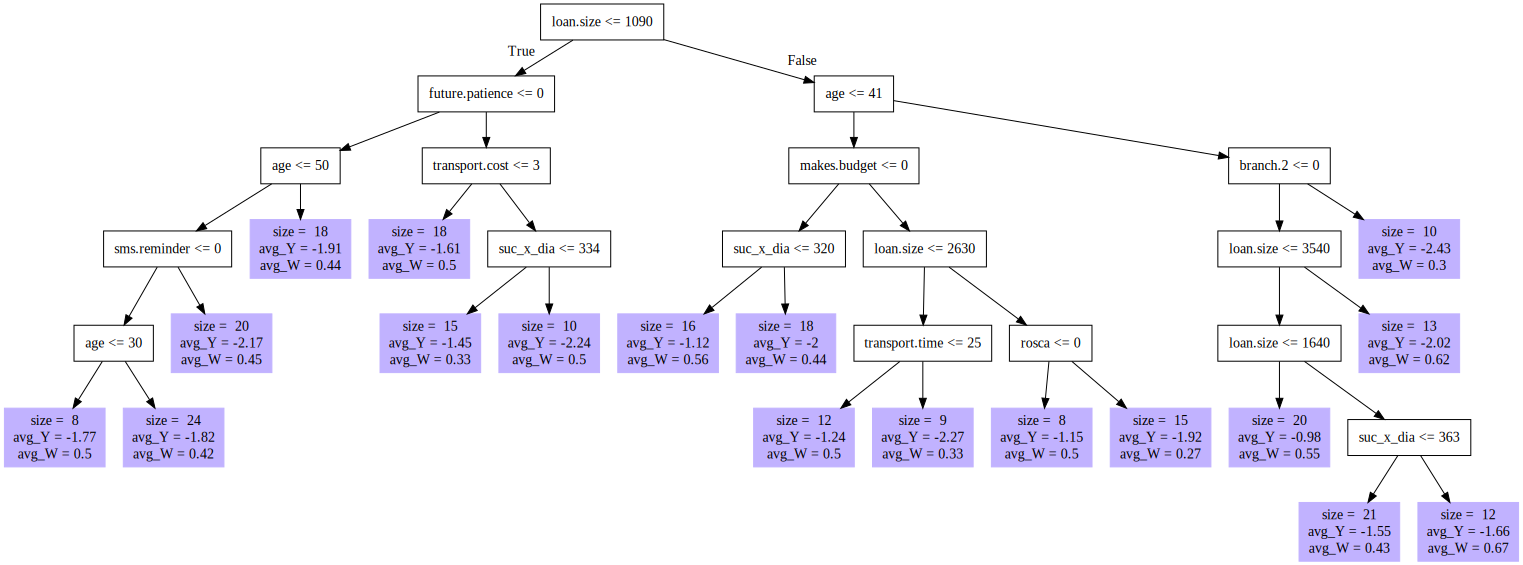
\includegraphics[width=\textwidth]{Figuras/crf_apr.pdf}
    \end{center}
    \legend{ 
    This figure shows an example of one of the regression trees used to compute the causal forest estimates described in Section \ref{sec:RF}. Each tree is constructed from a sequence of recursive binary partitions of the covariate space, with a splitting rule that is targeted to the causal quantity of interest, following the methodology of \cite{atheygrf}.}
    %This is one(it is chosen such that it minimizes the pruned cost, that is it is the tree with the smallest root-node impurity) of the honest causal trees in the random forest we use for the estimation of the heterogeneous treatment effect of the fee-forcing contract. It is meant only as an example of how these trees look like. The forest was such that there are as many estimated treatment effects as there are clients.
     %\footnotesize{ \textit{RScript: }  \texttt{grf.R}
\end{figure}


\begin{figure}[!htb]
    \begin{center}
  \caption{Cumulative Distribution Function of Conditional ATE Estimates}
  \includegraphics[width=0.7\textwidth]{Figuras/cdf_CATE.pdf} 
    \label{fig:CATEsurvival}
     \legend{This figure shows the share of borrowers who benefit from forced commitment, where ``benefit'' is defined as having an estimated conditional average treatment effect (ATE) above a specified threshold value. Results are based on the causal forest model from Section \ref{sec:RF}. The solid line equals $1 - F_\text{ATE}(\delta)$ where $F_\text{ATE}(\delta)$ denotes the CDF corresponding to the density of conditional ATE estimates from Figure \ref{heterogeneous_effects}. The blue shaded regions are associated 95\% confidence intervals. We estimate that at least 90\% of borrowers have a positive conditional ATE.}
    \end{center}
    
   
%\textit{Do file: }  \texttt{cdf_CATE.do}
\end{figure}
 


\begin{figure}[!htb]
    \caption{Conditional ATEs from ``wide'' and ``narrow'' covariate sets}
    \label{wide_narrow_forests}
    \begin{center}
    \begin{subfigure}{0.7\textwidth}
        \centering
        \includegraphics[width=\textwidth]{Figuras/scatter_hist_wide_narrow.pdf}
    \end{subfigure}
    \legend{This figure plots the relationship between the causal forest conditional ATE estimates from Section \ref{sec:RF} that use the ``wide'' set of covariates (all intake survey responses) and those based on a restricted ``narrow'' set of covariates (age, gender, HS education, and previous borrowing). The scatterplot graphs one estimate versus the other, with the ``wide'' covariate set on the horizontal axis and the ``narrow'' set on the vertical axis. The density plots on each axis show the estimated marginal distribution of conditional ATEs under each covariate set. The density for the ``wide'' covariate set is considerably more dispersed, as the causal forest based on this set of covariates captures considerably more treatment effect heterogeneity.}
    \end{center}
      

%\textit{Do file: } \texttt{wide_narrow_forests.do}       
\end{figure}







\subsection{Targeting rule comparisons}



\begin{figure}[!htb]
    \caption{Targeting rules}
    \label{targeting_rules}
    \begin{center}
    \begin{subfigure}{0.7\textwidth}
        \centering
        \includegraphics[width=\textwidth]{Figuras/wide_narrow_rule.pdf}
    \end{subfigure}
    \end{center}
      \legend{ This figure plots the percentage of borrowers who would benefit from a program in which commitment is targeted using the ``narrow'' covariate set (age, gender, HS education, and previous borrowing). In this exercise ``benefit'' is defined to mean having a conditional ATE above a particular threshold, taking the estimated conditional effects from the ``wide'' causal forest as ground truth. The plot compares the estimated percentage of borrowers who benefit, along with associated 95\% confidence bands, for three targeting rules: universal forced commitment in blue, targeting based on a random forest classification model in green, and targeting based on the logit model in red. For each of the classification models, the outcome variable is an indicator for whether the CATE estimate from the ``wide'' random forest model is positive. Each of the classification models produces an estimated probability of a positive CATE. For each, the assignment rule ranks borrowers by this estimated probability, and assigns the highest 90\% to forced commitment, to match the overall percentage of borrowers with positive estimated CATEs from the ``wide'' random forest model. Because this is an in-sample exercise, it overstates the actual performance of logit and RF-based targeting. }
     

\end{figure}


Figure \ref{targeting_rules} compares the in-sample performance of these targeting rules against a policy of universal forced commitment. The plot presents the estimated proportion of borrowers who benefit from a particular treatment assignment rule, along with associated 95\% confidence bands, where ``benefit'' is defined as having a conditional average treatment effect above a particular threshold. As above, we take the conditional average effects from the ``wide'' causal forest as ground truth for the purposes of this exercise. Because this is an in-sample exercise, the logistic and random forest classification rules have an unfair advantage: there is no adjustment for overfitting. In spite of this, their performance is quite unimpressive relative to a policy of universal forced commitment. The fraction of the whole sample incorrectly targeted when moving from universal forced commitment to targeting based on the narrow RF falls only from 9.78\% to 9.59\%. The logit targeting rule actually makes things marginally worse. 




\end{appendix}
